\documentclass[eng]{csam}
\usepackage{amsmath,amsfonts,amssymb,array,tabularx,enumerate}
\usepackage{epsfig, latexsym, natbib, graphicx, multirow}
\usepackage{bm,url,makecell}
\usepackage{algorithm,algorithmic}

%% ==================================================================
%% Manuscript prepared with the CSAM class file (csam.cls)
%% Communications for Statistical Applications and Methods
%% ==================================================================

%% ---- Submission (review) mode: line numbers, no journal header ----
\submit{draft}
\heading{Multivariate size-biased mixtures}

%% ---- Final (production) mode: comment out the two lines above and
%% ---- uncomment the block below; the journal office supplies the values.
%\submit{final}
%\volumn{VOL}{NO}{YEAR}{DATE}
%\receive{YYYY}{MM}{DD} \revise{YYYY}{MM}{DD} \accept{YYYY}{MM}{DD}
%\setpagenum{1}
%\heading{Multivariate size-biased mixtures}{Taehan Bae, Himchan Jeong}

%% ---- Author macros ------------------------------------------------
\def\a{\alpha}
\def\s{\sigma}
\def\argmax{\operatornamewithlimits{arg\,max}}
\def\mE{\mathbb{E}}
\def\mV{\text{Var}}
\def\mC{\text{Cov}}
\def\mP{\text{P}}
\renewcommand\cellalign{lc}

\begin{document}

\title{A multivariate extension of size-biased mixtures and its estimation using a penalized EM algorithm}

\author{Taehan Bae\footnote{Corresponding author: Department of Mathematics and Statistics, University of Regina, Regina, Saskatchewan, Canada. E-mail: taehan.bae@uregina.ca}\address[a]{Department of Mathematics and Statistics, University of Regina;}, Himchan Jeong\address[b]{Department of Statistics and Actuarial Science, Simon Fraser University}}

\begin{abstract}
Finite mixtures have been among the most widely used approaches for modeling complex data drawn from a population composed of heterogeneous sub-populations. In particular for insurance loss modelling, several mixtures of weighted distributions such as Erlang mixture, size-biased Weibull mixture and size-biased truncated lognormal mixture, have gained popularity due to the weak-denseness property.
This paper aims to extend univariate size-biased mixture models to multivariate cases. A penalized EM algorithm that facilitates the purging of statistically insignificant components, and thus results in a parsimonious model than the one fitted by the classical EM algorithm, is employed for model estimation. Three specific multivariate size-biased models: Erlang, size-biased Weibull and size-biased truncated lognormal models, are considered for model fitting on a real dataset.
\end{abstract}

\keywords{size-biased mixture, multivariate mixture, Erlang mixture, penalized EM algorithm, dependence modeling, insurance loss.}

\section{Introduction}
Finite mixture models (FMMs) have become a cornerstone of statistical modeling, providing a robust framework for analyzing data originating from heterogeneous populations. The foundational work of \citet{Titterington1985} established the strong theoretical underpinnings of FMMs and their wide-ranging applicability across diverse fields. \citet{Lindsay1995} further contributed to the understanding of FMMs, offering a comprehensive overview of their theory and applications, and highlighting their versatility in capturing complex data structures.

The appeal of FMMs lies in their ability to decompose a complex dataset into a mixture of simpler, more manageable components. By assuming that data points are drawn from a combination of underlying distributions, FMMs can effectively capture the heterogeneity present in the data and reveal the hidden population structures. This makes them particularly useful in situations where data points may belong to different subgroups, each with its own distinct characteristics.

In insurance loss modeling, the use of univariate FMMs has gained considerable traction, as demonstrated by the work of \citet{leelin2010} and \citet{Verbelen2015}. Their research showcases the effectiveness of Erlang mixtures in modeling claim data, capturing the skewness and heavy tails often observed in insurance loss distributions \citep{Klugman2019}. These characteristics are critical for accurately assessing risk and pricing insurance policies. In \citet{blostein2019modeling}, various finite mixtures with components from different parametric distribution families such as gamma, lognormal, Weibull and Burr distributions have been used for modelling left-truncated loss data. Finite mixtures have also been widely used in insurance ratemaking, for instance in the design of optimal bonus-malus systems \citep{tzougas2014optimal, tzougas2018bonus}, and robust estimation of heavy-tailed finite mixture models was studied by \citet{fung2022maximum}. More recently, \citet{fung2024soft} proposed the soft splicing model, which bridges the gap between composite models and finite mixture models for heavy-tailed loss data.

The work of \citet{bae2020mixtures} further underscores the flexibility of size-biased Weibull mixtures in modeling insurance loss data. Their findings reveal that size-biased Weibull mixtures outperform traditional models in capturing the tail behavior of insurance loss distributions, providing a more accurate assessment of large losses. This is particularly important for measuring the tail risks associated with insurance losses.

Building on this foundation, \citet{bae2024loss} introduce the size-biased truncated lognormal mixture, specifically tailored for left-truncated loss data. Left truncation occurs when data below a certain threshold is not observed, which is common in insurance settings where small claims may not be reported. The size-biased truncated lognormal mixture provides a more accurate representation of the loss distribution in such cases, leading to improved risk assessment and pricing.

Another line of research extends finite mixtures to the regression setting through the mixture-of-experts framework, in which the mixing weights depend on covariates. \citet{fung2019class_theory} studied the theoretical properties, including denseness, of the logit-weighted reduced mixture-of-experts (LRMoE) model, and \citet{fung2019class_freq} applied it to correlated claim frequencies. Severity regression versions of the model, including those for censored and truncated data, were developed by \citet{fung2021new} and \citet{fung2022fitting}, with a software implementation described in \citet{tseung2021lrmoe}. The framework was further extended with random effects by \citet{tseung2023improving} and to multilevel data by \citet{fung2025mixture}, while \citet{fung2023mixture} considered mixture composite regression models with multi-type feature selection.

While univariate FMMs have provided valuable insights, the extension to multivariate models has gained increasing momentum in recent years. Many real-world phenomena are characterized by multiple correlated variables, and capturing the relationships between these variables is essential for accurate modeling and prediction. Various multivariate mixture models beyond the Gaussian mixture have been investigated in \citet{Bouguila2020}. Their work highlights the potential of multivariate mixture models to uncover complex relationships between variables and to provide a more nuanced understanding of the underlying data structure. In actuarial domain, \citet{leelin2012} introduce a class of multivariate Erlang mixtures which extends the univariate Erlang mixture to higher dimensions. Dependence among insurance losses is more commonly modelled through copulas \citep{Frees1998, Klugman1999, jeong2020application, aradhye2024copula, ahn2026normal}; other approaches include dependent compound risk models \citep{jeong2020predictive}, models for heavy-tailed multi-peril losses \citep{yan2024dependence}, and multivariate mixed regression models for claim severities and counts \citep{chen2022em, jeong2023multivariate}.

Parameter estimation in mixture models often relies on the Expectation-Maximization (EM) algorithm \citep{dempster1977maximum}, which is also the standard estimation tool for many mixed and mixture models in actuarial science \citep{tzougas2020em, tzougas2021expectation, aradhye2024em}. However, EM can lead to overfitting, resulting in spurious model components. Penalized EM algorithms address this by encouraging the removal of insignificant components, leading to more parsimonious models \citep{Figueiredo}. For Erlang mixtures, \citet{yin2016efficient} proposed an iSCAD penalty to obtain parsimonious fits, and regularized estimation has also been applied to other actuarial problems such as the estimation of loss development factors \citep{jeong2021nonconvex}.

The present paper aims to develop a unified modelling framework for multivariate size-biased mixture model classes including the multivariate Erlang mixture class. We utilize a penalized EM algorithm to estimate parameters in our multivariate size-biased mixture model, carefully balancing model fit and complexity. By extending size-biased mixtures to the multivariate setting and employing penalized EM, we provide a valuable tool for complex data analysis, with particular relevance to insurance and related fields.

This paper is structured as follows: Section \ref{sec2} reviews univariate size-biased mixtures; Section \ref{sec3} introduces the framework for multivariate size-biased mixtures and derive expressions for some dependence measures; Section \ref{sec4} details the parameter estimation using the EM and the PEM algorithms. An application with a real bivariate loss data is given in Section \ref{sec5} followed by a concluding remarks in Section \ref{sec6}.


\section{Univariate size-biased mixtures}\label{sec2}
Size-biased distributions are a special case of weighted distributions, whose use in statistical modeling dates back to \citet{patil:1978}; see also \citet{gupta1990role}. Let a positive continuous random variable $X$ have an $M$-component mixture of size-biased (SB) distributions on a (parametric) baseline density function $h(x; \bm{\theta}),\, x >0$. Specifically the probability density function (pdf) of $X$ is expressed as
\begin{equation}\label{pdf_marginal}
f(x; \bm{\a}, \bm{\theta}) = \sum_{l = 1}^{M} \a_{l} g(x;s_l, \bm{\theta}),\quad x >0,
\end{equation}
where $\a_{l} \ge 0$ and $\sum_{l = 1}^{M} \a_{l} = 1$, and
\begin{equation}\label{sb_den}
g(x;s_l, \bm{\theta}) = \frac{x^{s_l -1} h(x; \bm{\theta})}{\mu(s_l -1; \bm{\theta})}.
\end{equation}
Here the SB orders $s_1 < s_2 < \cdots < s_{M}$ are positive integers (i.e., $s_l \in Z_+$), and $\mu(m; \bm{\theta}) := \int_0^{\infty} x^m h(x;\bm{\theta}) dx$ is the $m$-th raw moment of a random variable having the pdf $h$. Note that the parameter (vector) $\bm{\theta}$ is assumed to be common to all mixture components of $X$ for simplicity.

Three specific examples of size-biased mixture class available in the literature are (i) Erlang mixtures \citep{leelin2010, willmot2011risk, Verbelen2015} that are built on the exponential baseline density function $h(x;\theta) = \theta^{-1}\exp\{-x/\theta\}$, (ii) size-biased Weibull mixtures \citep{bae2020mixtures} constructed on the Weibull baseline density $h(x;\tau,\theta) = \tau \theta^{-\tau} x^{\tau-1}\exp\{-(x/\theta)^{\tau}\}$, and (iii) size-biased left-truncated lognormal mixtures \citep{bae2024loss} built on the left-truncated lognormal baseline density with a fixed left truncation threshold $d >0$ and the model parameter $\sigma >0$. The parameter $\mu$ in the lognormal distribution is set as $\mu = \log d$ for simplicity since it is unidentifiable in the presence of the SB orders in the size-biased components. This simplification renders the following the baseline density for the size-biased left-truncated lognormal mixtures
\begin{equation*}
h(x;\sigma) = \frac{2}{x\sigma\sqrt{2\pi}}\exp\left\{-\frac{1}{2\sigma^2}\left[\log(x/d)\right]^2\right\}.
\end{equation*}

The main theoretical characteristic of aforementioned size-biased mixture models is the weak-denseness property. Roughly speaking, any positive continuous distribution can be approximated with either Erlang mixture or size-biased Weibull (SBW) mixture at an arbitrary precision as the number of components gets large. The same argument holds for the size-biased left-truncated lognormal (SBtLN) mixture for any left truncated distributions.

\section{Multivariate size-biased mixtures}\label{sec3}

Let $\bm{X} = (X_1,\ldots, X_d)$ be a $d$-dimensional random vector on $\bm{R}_+^d = (0,\infty)^d$ where the marginal distribution of $X_k$ is a finite mixture of size-biased random variables with (distinct) SB orders $(s_1^{(k)}, s_2^{(k)}, \ldots, s_{M_k}^{(k)})$ along with other parameter (vector) $\bm{\theta}_k$ passed down from the baseline density. For each $k = 1,\ldots, d$, let us define a discrete random variable $J_k$ which attains a value from the set of SB orders, $S_{J_k} := \{s_1^{(k)}, s_2^{(k)}, \ldots, s_{M_k}^{(k)}\}$.

A $d$-dimensional random vector $\bm{J} = (J_1,\ldots, J_d)$ attains a grid point in $S_{\bm{J}} := \prod_{k=1}^d S_{J_k}$ where the total number of grid points in $S_{\bm{J}}$ is $M := \prod_{k=1}^d M_k$.

We further denote the joint probability of $\bm{J}$ by
\begin{equation*}
\a_{i_1,\ldots,i_d} := \mP\left(J_1 = s^{(1)}_{i_1}, \ldots, J_d = s^{(d)}_{i_d}\right)
\end{equation*}
where $i_k \in \{1,\ldots, M_k\}$ for each $k = 1,\ldots, d$.

Denoting $\bm{\Psi}$ the vector of all model parameters, we now write the joint density function of $\bm{X}$ as follows.
\begin{equation}\label{pdf_joint}
f(x_1,x_2,\ldots,x_d; \bm{\Psi}) = \sum_{i_1 = 1}^{M_1} \cdots\sum_{i_d = 1}^{M_d} \a_{i_1,i_2,\ldots,i_d} \prod_{k=1}^d g(x_k;s^{(k)}_{i_k}, \bm{\theta}_k).
\end{equation}
Therefore the joint distribution of $\bm{X}$ is a finite mixture of $M$ multivariate (independent) distributions.

Under this model specification, it is easy to see that the marginal distribution of $X_k$ is an $M_k$-point mixture of size-biased distributions, i.e.,
\begin{equation}\label{marginal_density}
f_k(x; \bm{\a}^{(k)}, \bm{\theta}_k) = \sum_{i_1 = 1}^{M_1} \cdots\sum_{i_d = 1}^{M_d} \a_{i_1,\ldots,i_d}g(x;s^{(k)}_{i_k},\bm{\theta}_k) = \sum_{l = 1}^{M_k} \a^{(k)}_{l} g(x;s^{(k)}_{l},\bm{\theta}_k),
\end{equation}
where
\begin{equation*}
\a^{(k)}_{l} = \sum_{i_1 = 1}^{M_1} \cdots \sum_{i_{k-1} = 1}^{M_{k-1}}\sum_{i_{k+1} = 1}^{M_{k+1}}\cdots \sum_{i_d = 1}^{M_d} \a_{i_1,\ldots,i_{k-1}, l, i_{k+1},\ldots, i_d}.
\end{equation*}

The joint density function of a pair $(X_u, X_v)$ is expressed as follows.
\begin{equation}\label{pair_density}
f_{u,v}(x, y; \bm{\a}^{(u,v)}, \bm{\theta}_u, \bm{\theta}_v) = \sum_{l = 1}^{M_u}\sum_{m = 1}^{M_v} \a^{(u,v)}_{l,m} g(x;s^{(u)}_{l},\bm{\theta}_u)g(y;s^{(v)}_{m},\bm{\theta}_v),
\end{equation}
where
\begin{multline*}
\a^{(u,v)}_{l,m} = \sum_{i_1 = 1}^{M_1} \cdots \sum_{i_{u-1} = 1}^{M_{u-1}}\sum_{i_{u+1} = 1}^{M_{u+1}}\cdots \sum_{i_{v-1} = 1}^{M_{v-1}}\sum_{i_{v+1} = 1}^{M_{v+1}}\cdots \sum_{i_d = 1}^{M_d}\\
\a_{i_1,\ldots,i_{u-1}, l, i_{u+1},\ldots, i_{v-1}, m, i_{v+1},\ldots, i_d}.
\end{multline*}

By (\ref{sb_den}) and (\ref{pdf_joint}), it is easy to obtain the following expression for the joint moment of $\bm{X}$.
\begin{align}
\mE\left[\prod_{k=1}^d X_{k}^{n_k}\right] &= \int_0^{\infty} \cdots \int_0^{\infty}\left(\prod_{k=1}^d x_{k}^{n_k}\right) f(x_1,x_2,\ldots,x_d; \bm{\Psi})\, dx_1\ldots dx_d \nonumber\\
&= \sum_{i_1 = 1}^{M_1} \cdots\sum_{i_d = 1}^{M_d} \a_{i_1,i_2,\ldots,i_d} \prod_{k=1}^d \left[\int_0^{\infty} x_k^{n_k}g(x_k;s^{(k)}_{i_k}, \bm{\theta}_k)\, dx_k\right] \nonumber\\
&= \sum_{i_1 = 1}^{M_1} \cdots\sum_{i_d = 1}^{M_d} \a_{i_1,i_2,\ldots,i_d} \prod_{k=1}^d \left[\frac{\mu(s^{(k)}_{i_k} + n_k -1; \bm{\theta}_k)}{\mu(s^{(k)}_{i_k} -1; \bm{\theta}_k)}\right]. \label{joint_mom}
\end{align}


\subsection{Dependence measures}
Here we give explicit expressions of some commonly used dependence measures for the bivariate size-biased mixture distribution: covariance, Spearman's rho and Kendall's tau.

\subsubsection{Covariance}

From the expression for the joint moment (\ref{joint_mom}), it is straightforward to obtain an expression for the covariance between two size-biased mixture random variables.

\begin{proposition}\label{prop:cov}
Suppose $(X_u, X_v)$ has the bivariate size-biased mixture distribution with the joint density function $f_{u,v}(x, y; \bm{\a}^{(u,v)}, \bm{\theta}_u, \bm{\theta}_v)$ (\ref{pair_density}), and the marginal densities $f_u(x; \bm{\a}^{(u)}, \bm{\theta}_u)$ and $f_v(x; \bm{\a}^{(v)}, \bm{\theta}_v)$ (\ref{marginal_density}), respectively for $X_u$ and $X_v$. Then the covariance is expressed as follows.
\begin{equation}
\mC[X_u, X_v] = \sum_{l = 1}^{M_u}\sum_{m = 1}^{M_v} \left(\a^{(u,v)}_{l,m} - \a^{(u)}_{l} \a^{(v)}_{m}\right)m(s_l^{(u)},\bm{\theta}_u)m(s_m^{(v)},\bm{\theta}_v),
\end{equation}
where
\begin{equation*}
m(s,\bm{\theta}) := \int_0^\infty x\, g(x;s,\bm{\theta})\,dx = \frac{\mu(s;\bm{\theta})}{\mu(s-1;\bm{\theta})}.
\end{equation*}
\end{proposition}

\noindent{\it Proof.} See Appendix \ref{app:props}.

\subsubsection{Spearman's rho}

The population version Spearman's rho ($\rho$) of random variables $T_1$ and $T_2$ with marginal densities $f_{T_1}(t_1)$ and $f_{T_2}(t_2)$, respectively, and the joint distribution $F(t_1, t_2)$ on $(0, \infty)\times (0, \infty)$, is defined as follows:
\begin{align}
\rho &= \frac{\mE[U_1 U_2] - \mE[U_1]\mE[U_2]}{\sqrt{\mV[U_1]}\sqrt{\mV[U_2]}} \nonumber\\
&= 12 \int_{0}^{\infty}\int_{0}^{\infty} F(t_1, t_2) f_{T_1}(t_1)f_{T_2}(t_2)\,dt_1 dt_2 -3, \label{def:rho}
\end{align}
where $U_1 = F_{T_1}(T_1)$ and $U_2 = F_{T_2}(T_2)$ are uniform random variables. The following gives an expression for the Spearman's rho of a pair $(X_u, X_v)$ with the joint density function (\ref{pair_density}).
\begin{proposition}\label{prop:rho}
Suppose $(X_u, X_v)$ has the bivariate size-biased mixture distribution with the joint density function $f_{u,v}(x, y; \bm{\a}^{(u,v)}, \bm{\theta}_u, \bm{\theta}_v)$ given in (\ref{pair_density}), and the marginal densities $f_u(x; \bm{\a}^{(u)}, \bm{\theta}_u)$ and $f_v(x; \bm{\a}^{(v)}, \bm{\theta}_v)$ given in (\ref{marginal_density}), respectively for $X_u$ and $X_v$. Then the Spearman's rho is expressed as follows.
\begin{equation}\label{rho_exp}
\rho = 12\sum_{l = 1}^{M_u}\sum_{m = 1}^{M_v} \sum_{l^\prime = 1}^{M_u}\sum_{m^\prime = 1}^{M_v} \a^{(u,v)}_{l,m} \a^{(u)}_{l^\prime}\a^{(v)}_{m^\prime} \lambda(s_l, s_{l^\prime}, \bm{\theta}_u)\lambda(s_m, s_{m^\prime}, \bm{\theta}_v) -3,
\end{equation}
where
\begin{equation*}
\lambda(s, t, \bm{\theta}) := \int_0^{\infty} G(x;s, \bm{\theta})g(x; t, \bm{\theta})\,dx.
\end{equation*}
Here $G(x;s, \bm{\theta}) := \int_0^x g(y; s, \bm{\theta})dy$ is the distribution function of the size-biased random variable with density (\ref{sb_den}).
\end{proposition}

\noindent{\it Proof.} See Appendix \ref{app:props}.

\subsubsection{Kendall's tau}

Kendall's tau ($\tau$) is often used as a measure of concordance between two random variables. Specifically, the population version Kendall's tau of continuous random variables $T_1$ and $T_2$ with marginal densities $f_{T_1}(t_1)$ and $f_{T_2}(t_2)$, respectively, and the joint distribution $F(t_1, t_2)$ on $(t_1, t_2) \in (0, \infty)\times (0, \infty)$, is defined as follows:
\begin{align}
\tau &= \mP[(T_1-T_1^{\prime})(T_2 - T_2^{\prime}) > 0] - \mP[(T_1-T_1^{\prime})(T_2 - T_2^{\prime}) < 0] \nonumber\\
&= 4 \int_{0}^{\infty}\int_{0}^{\infty} F(t_1, t_2) f(t_1, t_2)\,dt_1 dt_2 - 1, \label{def:tau}
\end{align}
where $(T_1, T_2)$ and $(T_1^{\prime}, T_2^{\prime})$ are independent and identically distributed random vectors each with the joint distribution $F$. Similarly as Spearman's rho, the following expression of Kendall's tau is available for a pair of size-biased mixture random variables.

\begin{proposition}\label{prop:tau}
Suppose $(X_u, X_v)$ has the bivariate size-biased mixture distribution with the joint density function $f_{u,v}(x, y; \bm{\a}^{(u,v)}, \bm{\theta}_u, \bm{\theta}_v)$ given in (\ref{pair_density}), and the marginal densities $f_u(x; \bm{\a}^{(u)}, \bm{\theta}_u)$ and $f_v(x; \bm{\a}^{(v)}, \bm{\theta}_v)$ given in (\ref{marginal_density}), respectively for $X_u$ and $X_v$. Then the Kendall's tau is expressed as follows.
\begin{equation}\label{tau_exp}
\tau = 4\sum_{l = 1}^{M_u}\sum_{m = 1}^{M_v} \sum_{l^\prime = 1}^{M_u}\sum_{m^\prime = 1}^{M_v} \a^{(u,v)}_{l,m} \a^{(u,v)}_{l^{\prime}, m^{\prime}} \lambda(s_l, s_{l^\prime}, \bm{\theta}_u)\lambda(s_m, s_{m^\prime}, \bm{\theta}_v) -1,
\end{equation}
where
\begin{equation*}
\lambda(s, t, \bm{\theta}) = \int_0^{\infty} G(x;s, \bm{\theta})g(x; t, \bm{\theta})\,dx.
\end{equation*}
\end{proposition}

\noindent{\it Proof.} See Appendix \ref{app:props}.

\medskip
Note that the expression $\lambda(s, t, \bm{\theta})$ involved in both (\ref{rho_exp}) and (\ref{tau_exp}) does not admit an explicit expression in general. For the Erlang mixture case where the baseline density is exponential, however, we have
\begin{align*}
g(x; t, \theta) &= \frac{x^{t-1}\exp[-x/\theta]}{\theta^t (t-1)!},\\
G(x; s, \theta) &= 1- \sum_{j=0}^{s-1}\frac{x^j \exp[-x/\theta]}{\theta^j j!}.
\end{align*}
Using these, it is easy to obtain the following explicit expression for $\lambda(s, t, \bm{\theta})$:
\begin{equation}\label{lambda_erlang}
\lambda(s, t, \theta) = 1- \sum_{j=0}^{s-1}\binom{j+t-1}{j}\left(\frac{1}{2}\right)^{j+t}.
\end{equation}


\subsubsection{Upper tail dependence}
Two random variables $X_u$ and $X_v$ having the bivariate size-biased mixture distribution are upper tail independent. That is,
\begin{align*}
\lambda_U &= \lim_{q\rightarrow 1}\mP\left[X_u > F^{-1}_u(q)\big{|}X_v > F^{-1}_v(q)\right]\\
&= \lim_{q\rightarrow 1}\frac{1- \mP[X_u \le F^{-1}_u(q)] - \mP[X_v \le F^{-1}_v(q)] + \mP[X_u \le F^{-1}_u(q), X_v \le F^{-1}_v(q)]}{1-q}\\
&= \lim_{q\rightarrow 1}\frac{1-2q + F_{u,v}(F^{-1}_u(q),F^{-1}_v(q))}{1-q} = 0,
\end{align*}
where $F_{u,v}(x,y)$ is the bivariate joint distribution function given in (\ref{pair_density}). It is elementary to show the above result using the ordering of the size-biased components. See Appendix \ref{app:tail} for details.


\section{Parameter estimation}\label{sec4}
\subsection{EM algorithm}\label{em}
The Expectation-Maximization (EM) algorithm \citep{dempster1977maximum} is widely used for the maximum likelihood estimation of finite mixture models in which each observation is generated from a randomly selected distribution out of a set of distributions with (prior) selection probabilities.

Let $\bm{x} := \{\bm{x}_1, \ldots, \bm{x}_n\}$ be a set of independent observations drawn from the joint distribution with the pdf (\ref{pdf_joint}). The vector of model parameters, $\bm{\Psi} = (\bm{\a}, \bm{\Theta})$, is composed of the vector of mixture weight parameters $\bm{\a}$ and all parameters involved in the baseline density functions $\bm{\Theta} = (\bm{\theta}_1,\ldots, \bm{\theta}_d)$. Denote $Z_{i,\bm{j}} : = Z_{i, (j_1,\ldots,j_d)}$ as the membership indicator random variable that takes the value 1 if the $i$th observation $\bm{x}_i = (x_{i1},\ldots,x_{id})$ is generated from the component with the vector of SB orders $(s^{(1)}_{j_1},\ldots, s^{(d)}_{j_d}) \in S_{\bm{J}}$, zero otherwise.

Then the complete log-likelihood function becomes
\begin{equation*}
l_c(\bm{\Psi}|\bm{x}) = \sum_{i=1}^n \sum_{j_1 = 1}^{M_1} \cdots\sum_{j_d = 1}^{M_d} Z_{i,\bm{j}}\left[\log(\a_{j_1,j_2,\ldots,j_d}) + \sum_{k=1}^d \log g(x_{ik};s^{(k)}_{j_k}, \bm{\theta}_k)\right].
\end{equation*}
The E-step of the EM algorithm computes $Q(\bm{\Psi};\bm{\Psi}^{old}) = \mE[l_c(\bm{\Psi}) |\bm{x}, \bm{\Psi}^{old}]$ where the expectation is taken with respect to the posterior probability of the membership indicator random variable $Z_{i,\bm{j}}$ given as
\begin{equation*}
\a_{i,(j_1,\ldots,j_d)} : = P(Z_{i,\bm{j}} = 1 | \bm{x}_i, \bm{\Psi}^{old}) = \frac{\a^{old}_{j_1,j_2,\ldots,j_d} \prod_{k=1}^d g(x_{ik};s^{(k)}_{j_k}, \bm{\theta}^{old}_k)}{\sum_{l_1 = 1}^{M_1} \cdots\sum_{l_d = 1}^{M_d}\a^{old}_{l_1,l_2,\ldots,l_d} \prod_{k=1}^d g(x_{ik};s^{(k)}_{l_k}, \bm{\theta}^{old}_k)}.
\end{equation*}
The M-step of the EM algorithm consists of maximizing the following Q-function to obtain the updated parameter estimates
\begin{align}
Q(\bm{\Psi};\bm{x}, \bm{\Psi}^{old}) &= \sum_{i=1}^n \sum_{j_1 = 1}^{M_1} \cdots\sum_{j_d = 1}^{M_d} \a_{i,(j_1,\ldots,j_d)}\left[\log \a_{j_1,j_2,\ldots,j_d} + \sum_{k=1}^d \log g(x_{ik};s^{(k)}_{j_k}, \bm{\theta}_k)\right] \nonumber\\
&= Q_1(\bm{\a};\bm{\Psi}^{old}) + Q_2(\bm{\theta}_1,\ldots, \bm{\theta}_d;\bm{\Psi}^{old}), \label{Estep}
\end{align}
where
\begin{align*}
Q_1(\bm{\a};\bm{\Psi}^{old}) &= \sum_{j_1 = 1}^{M_1} \cdots\sum_{j_d = 1}^{M_d} \left(\sum_{i=1}^n \a_{i,(j_1,\ldots,j_d)}\right)\log \a_{j_1,j_2,\ldots,j_d},\\
Q_2(\bm{\theta}_1,\ldots, \bm{\theta}_d;\bm{\Psi}^{old}) &= \sum_{i=1}^n \sum_{j_1 = 1}^{M_1} \cdots\sum_{j_d = 1}^{M_d} \a_{i,(j_1,\ldots,j_d)}\sum_{k=1}^d \log g(x_{ik};s^{(k)}_{j_k}, \bm{\theta}_k).
\end{align*}

By the Lagrange multiplier we can obtain an explicit solution for the maximization of $Q_1$. For each $\bm{j} = (j_1,j_2,\ldots,j_d)$, the estimate of the mixture weight parameter is
\begin{equation*}
\hat{\a}_{\bm{j}} = \hat{\a}_{j_1,j_2,\ldots,j_d} = \frac{1}{n} \sum_{i=1}^n \a_{i,(j_1,j_2,\ldots,j_d)}.
\end{equation*}

The maximization of $Q_2$ depends on the specific form of the size-biased component density function $g$.

In particular, the Erlang mixture component has the pdf, $g(x; s, \theta) = \theta^{-s} x^{s-1}e^{-x/\theta}/(s-1)!$. In this case we can obtain the following closed form expression for $\theta_k$:
\begin{equation*}
\hat{\theta}_k = \frac{\sum_{i=1}^n x_{ik}}{n \sum_{j_1 = 1}^{M_1} \cdots\sum_{j_d = 1}^{M_d} \a_{i,(j_1,\ldots,j_k, \ldots, j_d)}s^{(k)}_{j_k}},\quad k=1,\ldots, d.
\end{equation*}

The size-biased Weibull (SBW) distribution extends the Erlang distribution with an additional shape parameter $\tau >0$ whose density function is given as
\begin{equation*}
g(x;s, \tau, \theta) = \frac{\tau \theta^{-(\tau+ s -1)} x^{\tau + s -2}e^{-(x/\theta)^{\tau}}}{\Gamma[1+(s-1)/\tau]}.
\end{equation*}
In this case the updated estimate for $\theta_k$ in the SBW mixture distribution is given as
\begin{equation*}
\hat{\theta}_k = \left[\frac{\hat{\tau}_k \sum_{i=1}^n x^{\hat{\tau}_k}_{ik}}{n\left(\hat{\tau}_k-1 + \sum_{j_1 = 1}^{M_1} \cdots\sum_{j_d = 1}^{M_d} \a_{i,(j_1,\ldots,j_d)} s^{(k)}_{j_k}\right)}\right]^{1/\hat{\tau}_k},\quad k = 1,\ldots, d,
\end{equation*}
where $\hat{\tau}_k$ is the solution of the following optimization problem:
\begin{equation*}
\hat{\tau}_k = \argmax_{\tau_k} \sum_{i=1}^n \sum_{j_1 = 1}^{M_1} \cdots\sum_{j_d = 1}^{M_d} \a_{i,(j_1,\ldots,j_d)}\log g(x_{ik};s^{(k)}_{j_k}, \tau_k,\hat{\theta}_k),\quad k = 1,\ldots, d.
\end{equation*}
Due to the complexity of the objective function, a numerical method is required to solve this problem.

The size-biased left-truncated lognormal distribution has the following the density function
\begin{equation*}
g(x;s, \sigma) = \frac{x^{s-2}\exp\left\{-\frac{1}{2\s^2}\left[\log(x/d)\right]^2\right\}}{\sigma \sqrt{2\pi} d^{s-1}\exp\left\{(s-1)^2 \s^2 /2\right\}\Phi[(s-1)\sigma]},
\end{equation*}
where $\Phi[\cdot]$ denotes the standard normal cdf. In this case the updated estimate for $\sigma_k$ in the SBtLN mixture distribution is the solution of the following equation:
\begin{align*}
\frac{d Q_2}{d \sigma_k} &= - \frac{n}{\sigma_k} + \frac{1}{\sigma^3_k} \sum_{i=1}^n\left[\log (x_{ik}/d)\right]^2 - n \sigma_k \sum_{j_1 = 1}^{M_1} \cdots\sum_{j_d = 1}^{M_d} \a_{i,(j_1,\ldots,j_d)} (s^{(k)}_{j_k} -1)^2\\
&\qquad - n\sum_{j_1 = 1}^{M_1} \cdots\sum_{j_d = 1}^{M_d} \a_{i,(j_1,\ldots,j_d)} \frac{(s^{(k)}_{j_k} -1)\phi[(s^{(k)}_{j_k} -1)\sigma_k]}{\Phi[(s^{(k)}_{j_k} -1)\sigma_k]} = 0,\quad k=1,\ldots,d,
\end{align*}
where $\phi[\cdot]$ denotes the standard normal density function.

\subsection{Penalized EM algorithm}
The performance of the estimated multivariate model largely depends on the number of components in the fitted mixture model. It is often observed that the fitted models based on the classical EM algorithm involve spurious or redundant components with near zero mixture weight estimates. Here we consider a penalized EM algorithm (PEM) to facilitate purging of statistically insignificant components, which results in a simpler model than the one fitted by the classical EM algorithm. See \citet{Figueiredo} for details on the statistical learning of finite mixture models with various EM-based methods, and \citet{yin2016efficient} for a penalized approach to Erlang mixtures.

Specifically we aim to maximize the following penalized log-likelihood function
\begin{equation}\label{eq:pl}
Pl(\bm{\Psi}|\bm{x}) = l(\bm{\Psi}|\bm{x}) - \gamma n R(\bm{\a}),
\end{equation}
where $R(\bm{\a}) = \sum_{j_1 = 1}^{M_1} \cdots\sum_{j_d = 1}^{M_d}\log \a_{j_1,j_2,\ldots,j_d}$ and $\gamma > 0$ is the tuning parameter that controls the degree of penalty. Clearly the penalty gets its minimum (or $-\infty$) when the mixture weights for some components become zero. That is, the model maximizing the penalized log-likelihood function tends to drop some statistically insignificant (or spurious) components. In fact, from a Bayesian perspective, (\ref{eq:pl}) can be obtained by assuming Dirichlet-type prior for $\bm{\a}$ and other model parameters are assumed constant. Specifically, we assume the prior density of $\bm{\a}$ as
\begin{equation*}
p(\bm{\a}) \propto \prod_{j_1 = 1}^{M_1} \cdots\prod_{j_d = 1}^{M_d}\left(\a_{j_1,j_2,\ldots,j_d}\right)^{-\gamma n }.
\end{equation*}
Then the logarithm of the posterior density (up to a constant) is given as (\ref{eq:pl}).

With this specification, the PEM facilitates the mixture model to become parsimonious by encouraging some mixture weight parameter values to attain the value of zero. The PEM algorithm gives the following expectation step on the complete-data penalized log-likelihood function and the current parameter estimates
\begin{align}
\tilde{Q}(\bm{\Psi};\bm{x}, \bm{\Psi}^{old}) &= \sum_{i=1}^n \sum_{j_1 = 1}^{M_1} \cdots\sum_{j_d = 1}^{M_d} \a_{i,(j_1,\ldots,j_d)}\left[\log \a_{j_1,j_2,\ldots,j_d} + \sum_{k=1}^d \log g(x_{ik};s^{(k)}_{j_k}, \bm{\theta}_k)\right] \nonumber\\
&\qquad - \gamma n \sum_{j_1 = 1}^{M_1} \cdots\sum_{j_d = 1}^{M_d}\log \a_{j_1,j_2,\ldots,j_d} \nonumber\\
&= \tilde{Q}_1(\bm{\a};\bm{\Psi}^{old}) + \tilde{Q}_2(\bm{\theta}_1,\ldots, \bm{\theta}_d;\bm{\Psi}^{old}), \label{rEstep}
\end{align}
where
\begin{align*}
\tilde{Q}_1(\bm{\a};\bm{\Psi}^{old}) &= \sum_{j_1 = 1}^{M_1} \cdots\sum_{j_d = 1}^{M_d} \left(\sum_{i=1}^n (\a_{i,(j_1,\ldots,j_d)}-\gamma)\right) \log \a_{j_1,j_2,\ldots,j_d},\\
\tilde{Q}_2(\bm{\theta}_1,\ldots, \bm{\theta}_d;\bm{\Psi}^{old}) &= \sum_{i=1}^n \sum_{j_1 = 1}^{M_1} \cdots\sum_{j_d = 1}^{M_d} \a_{i,(j_1,\ldots,j_d)}\sum_{k=1}^d \log g(x_{ik};s^{(k)}_{j_k}, \bm{\theta}_k).
\end{align*}
With the constraints on the mixture weight parameters, $\a_{j_1,j_2,\ldots,j_d} \ge 0$ and $\sum_{j_1 = 1}^{M_1} \cdots\sum_{j_d = 1}^{M_d} \a_{j_1,j_2,\ldots,j_d} = 1$, the method of Lagrange multiplier renders an explicit solution for the maximization of $\tilde{Q}_1$. For each $\bm{j} = (j_1,j_2,\ldots,j_d)$, the updated estimate of the mixture weight parameter is given as
\begin{equation*}
\hat{\a}^{R}_{j_1,j_2,\ldots,j_d} = \frac{\max\{\sum_{i=1}^n \left(\a_{i,(j_1,j_2,\ldots,j_d)}-\gamma\right), 0\}}{\sum_{j_1 = 1}^{M_1} \cdots\sum_{j_d = 1}^{M_d} \max\{\sum_{i=1}^n \left(\a_{i,(j_1,j_2,\ldots,j_d)}-\gamma\right), 0\}}.
\end{equation*}
That is, the estimate $\hat{\a}^{R}_{j_1,j_2,\ldots,j_d} = 0$ when $n^{-1}\sum_{i=1}^n \a_{i,(j_1,j_2,\ldots,j_d)} \le \gamma$. In other words, the higher the tuning parameter $\gamma$, the simpler becomes the fitted model. Note that $\tilde{Q}_2(\bm{\theta}_1,\ldots, \bm{\theta}_d;\bm{\Psi}^{old})$ is identical to $Q_2(\bm{\theta}_1,\ldots, \bm{\theta}_d;\bm{\Psi}^{old})$ in (\ref{Estep}), and thus the estimation of $\bm{\theta}_k$ can be proceeded as in Section \ref{em}.


\subsection{Parameter initialization}\label{initial}
The EM based estimation methods suffer from their sensitivity to the initial parameter values. Random sets of parameter values may be used repeatedly until get the optimal result. For high-dimensional case with a large number of components, the randomization method is computationally intense. The stochastic ordering structure and the weak-denseness property can help alleviate the computational burden in parameter initialization.
Specifically for the univariate SBW mixture model, we proceed as follows. For each $\tau^{(0)}$,
\begin{equation*}
\theta^{(0)} = \frac{X_{(n)}}{(M/\tau)^{1/\tau}}, \qquad \a_j^{(0)} = \frac{1}{n}\sum_{i=1}^n I\left[\theta(s_{j-1}/\tau)^{1/\tau} < X_i \le \theta(s_j/\tau)^{1/\tau}\right].
\end{equation*}
Fit each marginal model using the EM (or PEM) algorithm. Use the estimated parameters for the initial values for the estimation of multivariate models. The weight parameters can be initialized as (Bivariate SBW mixture case for example)
\begin{align*}
\a_{l,m}^{(0)} = \frac{1}{n}\sum_{i=1}^n I\Big[ & \theta_1(s^{(1)}_{l-1}/\tau_1)^{1/\tau_1} < X_i \le \theta_1(s^{(1)}_l/\tau_1)^{1/\tau_1},\\
& \theta_2(s^{(2)}_{m-1}/\tau_2)^{1/\tau_2} < Y_{i} \le \theta_2(s^{(2)}_m/\tau_2)^{1/\tau_2}\Big].
\end{align*}

\begin{algorithm}[t]
\caption{Penalized EM algorithm}\label{alg:pem}
For a fixed tuning parameter $\gamma$:
\begin{itemize}
\item [] \underline{Parameter initialization}
\item [] \textbf{While} the stopping criterion is not satisfied \textbf{do}\\
\underline{E-Step}\\
Calculate posterior probabilities for each $i$ and $j = (j_1,j_2,\ldots,j_d)$:
\begin{equation*}
\a^{(r)}_{i,j} = \frac{\a^{(r-1)}_{j} \prod_{k=1}^d g(x_{ik};s^{(k)}_{j_k}, \bm{\theta}^{(r-1)}_k)}{\sum_{l_1 = 1}^{M_1} \cdots\sum_{l_d = 1}^{M_d}\a^{(r-1)}_{(l_1,l_2,\ldots,l_d)} \prod_{k=1}^d g(x_{ik};s^{(k)}_{l_k}, \bm{\theta}^{(r-1)}_k)}.
\end{equation*}
Given the parameter estimates $\bm{\Psi}^{(r-1)} = (\bm{\a}^{(r-1)}, \bm{\Theta}^{(r-1)})$ obtained in the $(r-1)$th iteration, establish $\tilde{Q}$-function:
\begin{equation*}
\tilde{Q}(\bm{\Psi};\bm{\Psi}^{(r-1)}) = \tilde{Q}_1(\bm{\a};\bm{\Psi}^{(r-1)}) + \tilde{Q}_2(\bm{\Theta};\bm{\Psi}^{(r-1)}).
\end{equation*}
\underline{M-Step}
\begin{align*}
\bm{\a}^{(r)} &\leftarrow \argmax_{\bm{\a}} \tilde{Q}_1(\bm{\a};\bm{\Psi}^{(r-1)}): \bm{\a}^{(r)}_{j} = \frac{\max\{\sum_{i=1}^n \left(\a^{(r)}_{i,j}-\gamma\right), 0\}}{\sum_{j_1 = 1}^{M_1}\cdots\sum_{j_d = 1}^{M_d} \max\left\{\sum_{i=1}^n \left(\a^{(r)}_{i,(j_1,j_2,\ldots,j_d)}-\gamma\right), 0 \right\}},\\
\bm{\Theta}^{(r)} &\leftarrow \argmax_{\bm{\Theta}} \tilde{Q}_2(\bm{\Theta};\bm{\Psi}^{(r-1)}).
\end{align*}
Calculate the criterion e.g., $D \leftarrow |\bm{\Theta}^{(r)} - \bm{\Theta}^{(r-1)}|_1$ \\
$\bm{\Psi}^{(r)} \leftarrow (\bm{\a}^{(r)}, \bm{\Theta}^{(r)})$\\
\textbf{end}\\
\textbf{return} $\bm{\Psi} = (\bm{\a}, \bm{\Theta})$.
\end{itemize}
Use the Bayesian information criterion (BIC) to select the optimal value of $\gamma$ on the grid of possible values.
\end{algorithm}


\section{Application}\label{sec5}
In this section we consider a liability claims dataset consisting of 1500 randomly selected bivariate observations of the indemnity payment (Loss) and the allocated loss adjustment expense (ALAE) \citep{Klugman1999}. We divide both variables by 1000 to have similar scales.

\begin{table}[t]
\footnotesize
\centering
\caption{Summary statistics of Loss and ALAE (unit: 1,000 USD)}\label{tab_data}
\begin{tabular}{ccccccccc}
\hline\hline
Variable & Min. & 1st Qu. & Median & Mean & 3rd Qu. & Max. & Skewness & Excess Kurtosis \\
\hline
Loss & 0.01 & 4.00 & 12.00 & 41.21 & 35.00 & 2173.59 & 9.15 & 141.98 \\
ALAE & 0.015 & 2.33 & 5.47 & 12.59 & 12.572 & 501.86 & 9.24 & 124.55 \\
\hline\hline
\end{tabular}
\end{table}

Table \ref{tab_data} gives basic summary statistics of each marginal. The high excess kurtosis suggests that both variables exhibit heavy tails. Figure \ref{scatterplots} presents scatterplots of the bivariate observations and their log-transformed versions to show a clear positive dependence between the two variables. The empirical dependence measures are 0.4022 (Pearson's correlation), 0.4519 (Spearman's rho), and 0.3154 (Kendall's tau).

\begin{figure}[t]
\centering
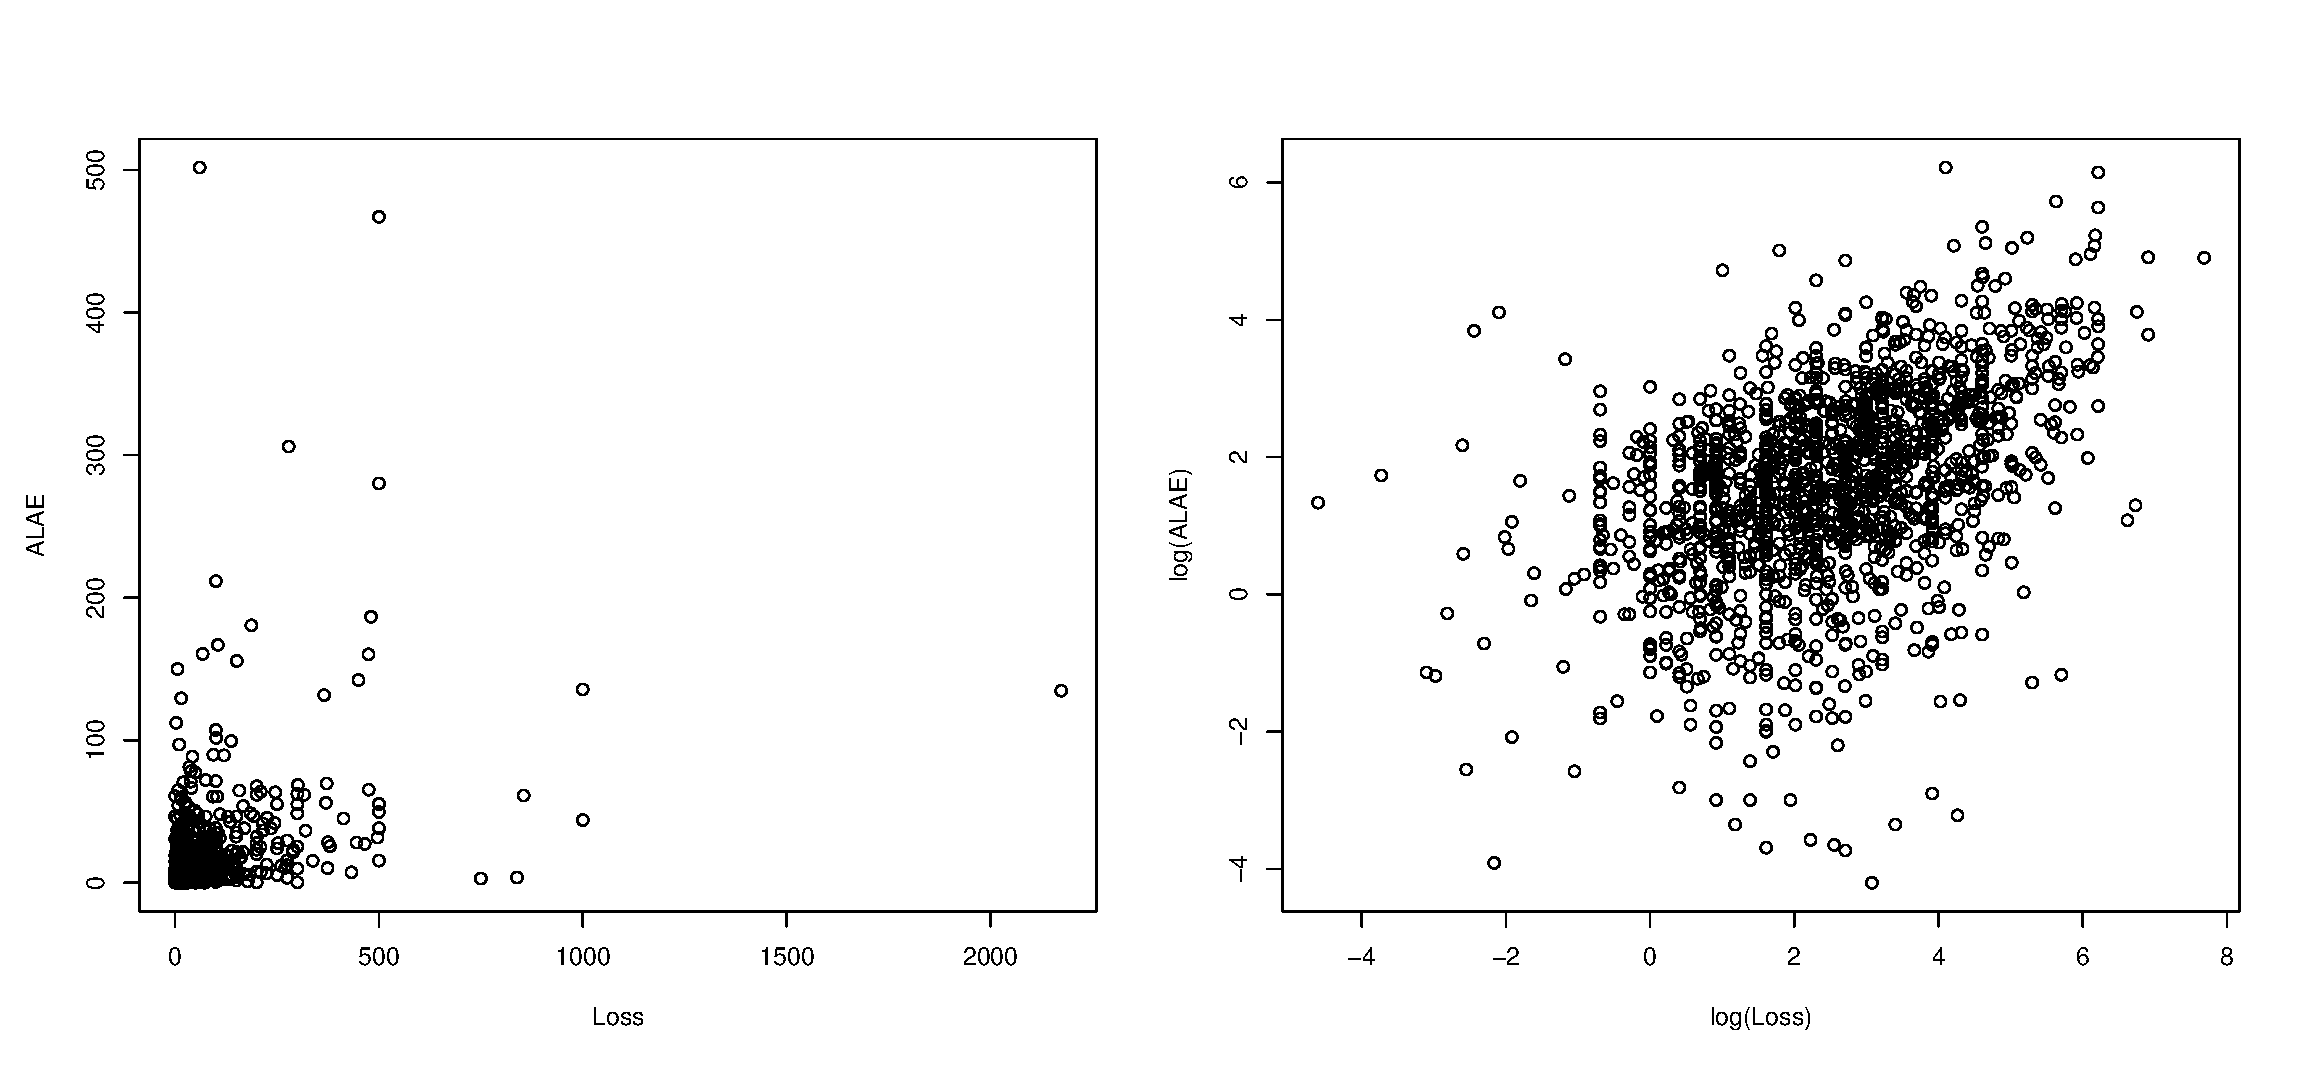
\includegraphics[height=5cm,keepaspectratio=true]{Loss_Alae_scatterplot.eps}
\caption{Scatter plots of the bivariate data (left) and its log-transformation (right)}
\label{scatterplots}
\end{figure}

For the estimation of the bivariate SB models, we first use the EM algorithm to fit the three size-biased mixture distributions, Erlang, SBW and SBtLN mixtures for each marginal. For each model, we employ the parameter initialization method relying on the weak-denseness property and stochastic ordering as described in Section \ref{initial}, and the best fit model is selected using the BIC. Table \ref{tab_marginal_fit} gives the negative log-likelihood value (NLL), the BIC value, the orders of the components in the best fit mixture model, and model parameter estimates for each model class. Figure \ref{denplots} presents the density curves (red colored) of the fitted size-biased mixture models on the data histograms. The results show that, overall the SBtLN model fits both marginals the best in terms of the Bayesian information criterion while the Erlang mixture tends to overfit the tail observations.

\begin{table}[t]
\footnotesize
\centering
\caption{Fitted univariate size-biased mixture models on each marginal variable}\label{tab_marginal_fit}
\begin{tabular}{lllll}
\hline\hline
Model & NLL & BIC & Component SB order & Parameter estimate \\
\hline
\multicolumn{5}{c}{Loss} \\
\hline
Erlang & 6600.88 & 13340.72 & 1 -- 15, 23, 26, 30, 65 & $\hat{\theta} = 14.47$ \\
SBW & 6596.20 & 13250.91 & 1 -- 4, 6, 7, 11 & $(\hat{\tau}, \hat{\theta}) = (0.766, 17.55)$ \\
SBtLN & 6560.05 & 13171.28 & 1 -- 7 & $\hat{\sigma} =1.325$ \\
\hline
\multicolumn{5}{c}{ALAE} \\
\hline
Erlang & 5053.27 & 10238.18 & 1 -- 9, 11, 12, 13, 15, 17, 22, 24, 37, 39 & $\hat{\theta} = 7.66$ \\
SBW & 5067.64 & 10201.10 & 1 -- 6, 8, 13 & $(\hat{\tau}, \hat{\theta}) = (0.867, 8.078)$ \\
SBtLN & 5054.73 & 10160.65 & 1 -- 7 & $\hat{\sigma} =1.243$ \\
\hline\hline
\end{tabular}
\end{table}

\begin{figure}[t]
\centering
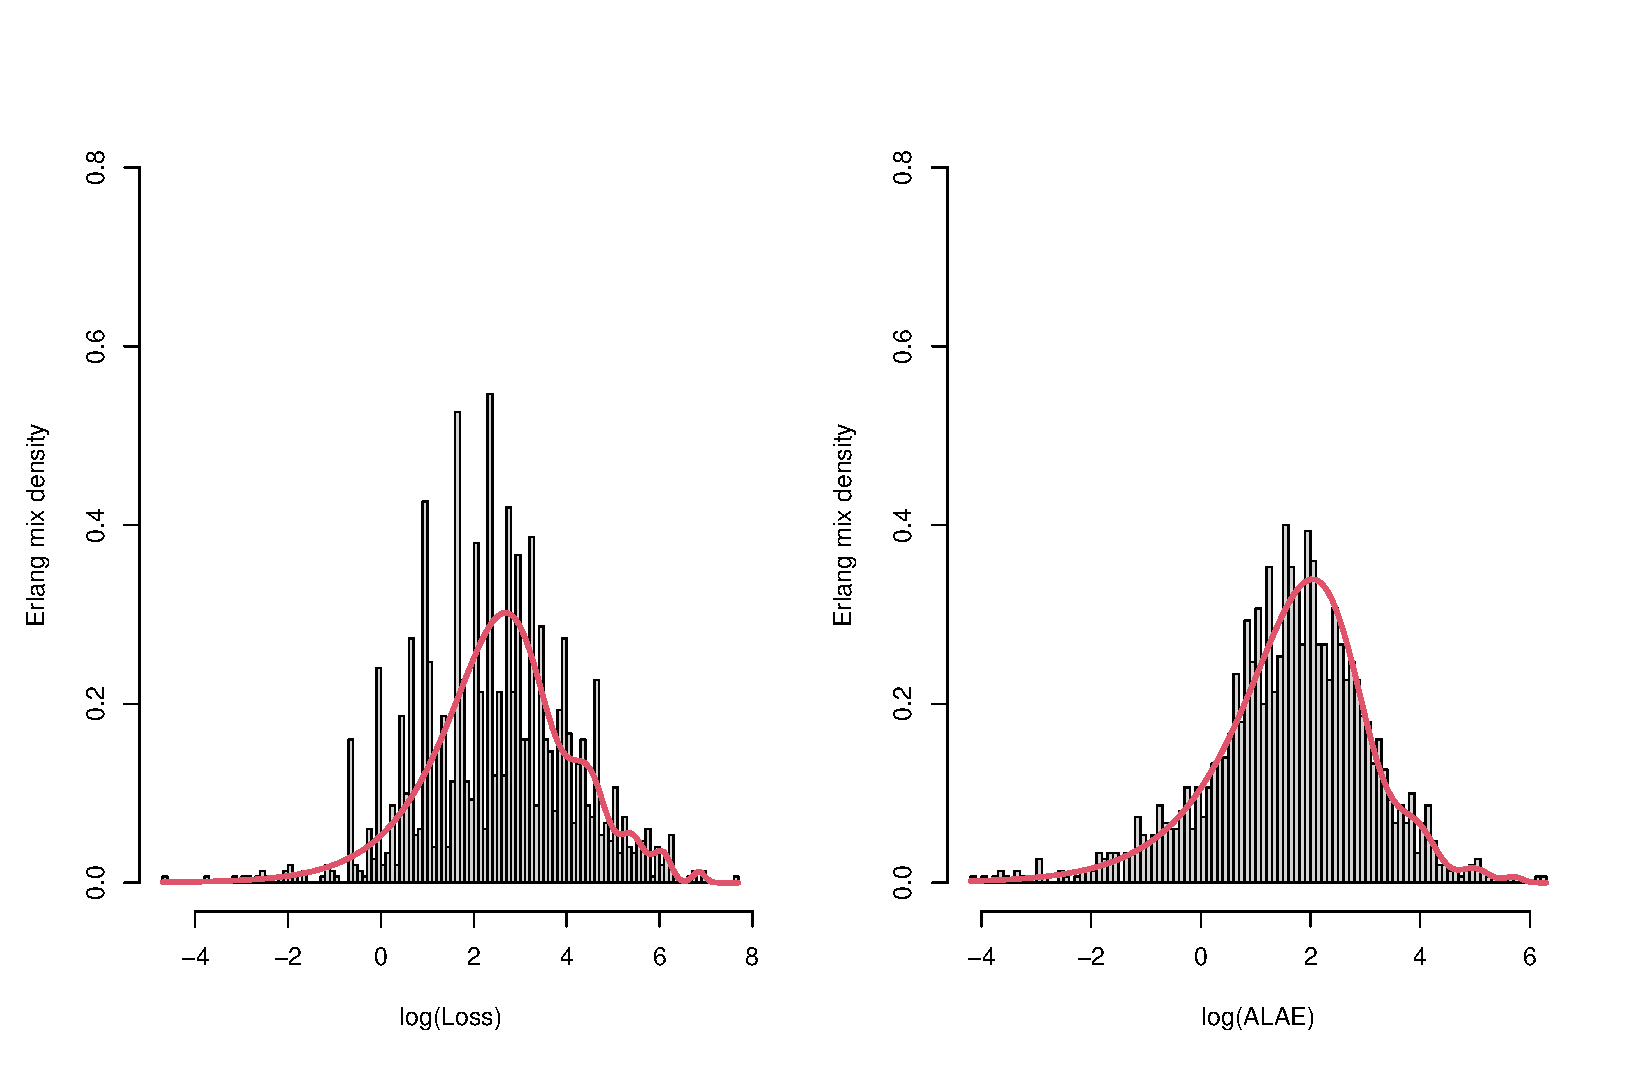
\includegraphics[height=5cm,keepaspectratio=true]{Loss_Alae_ErlangMargin_fit.eps}\\
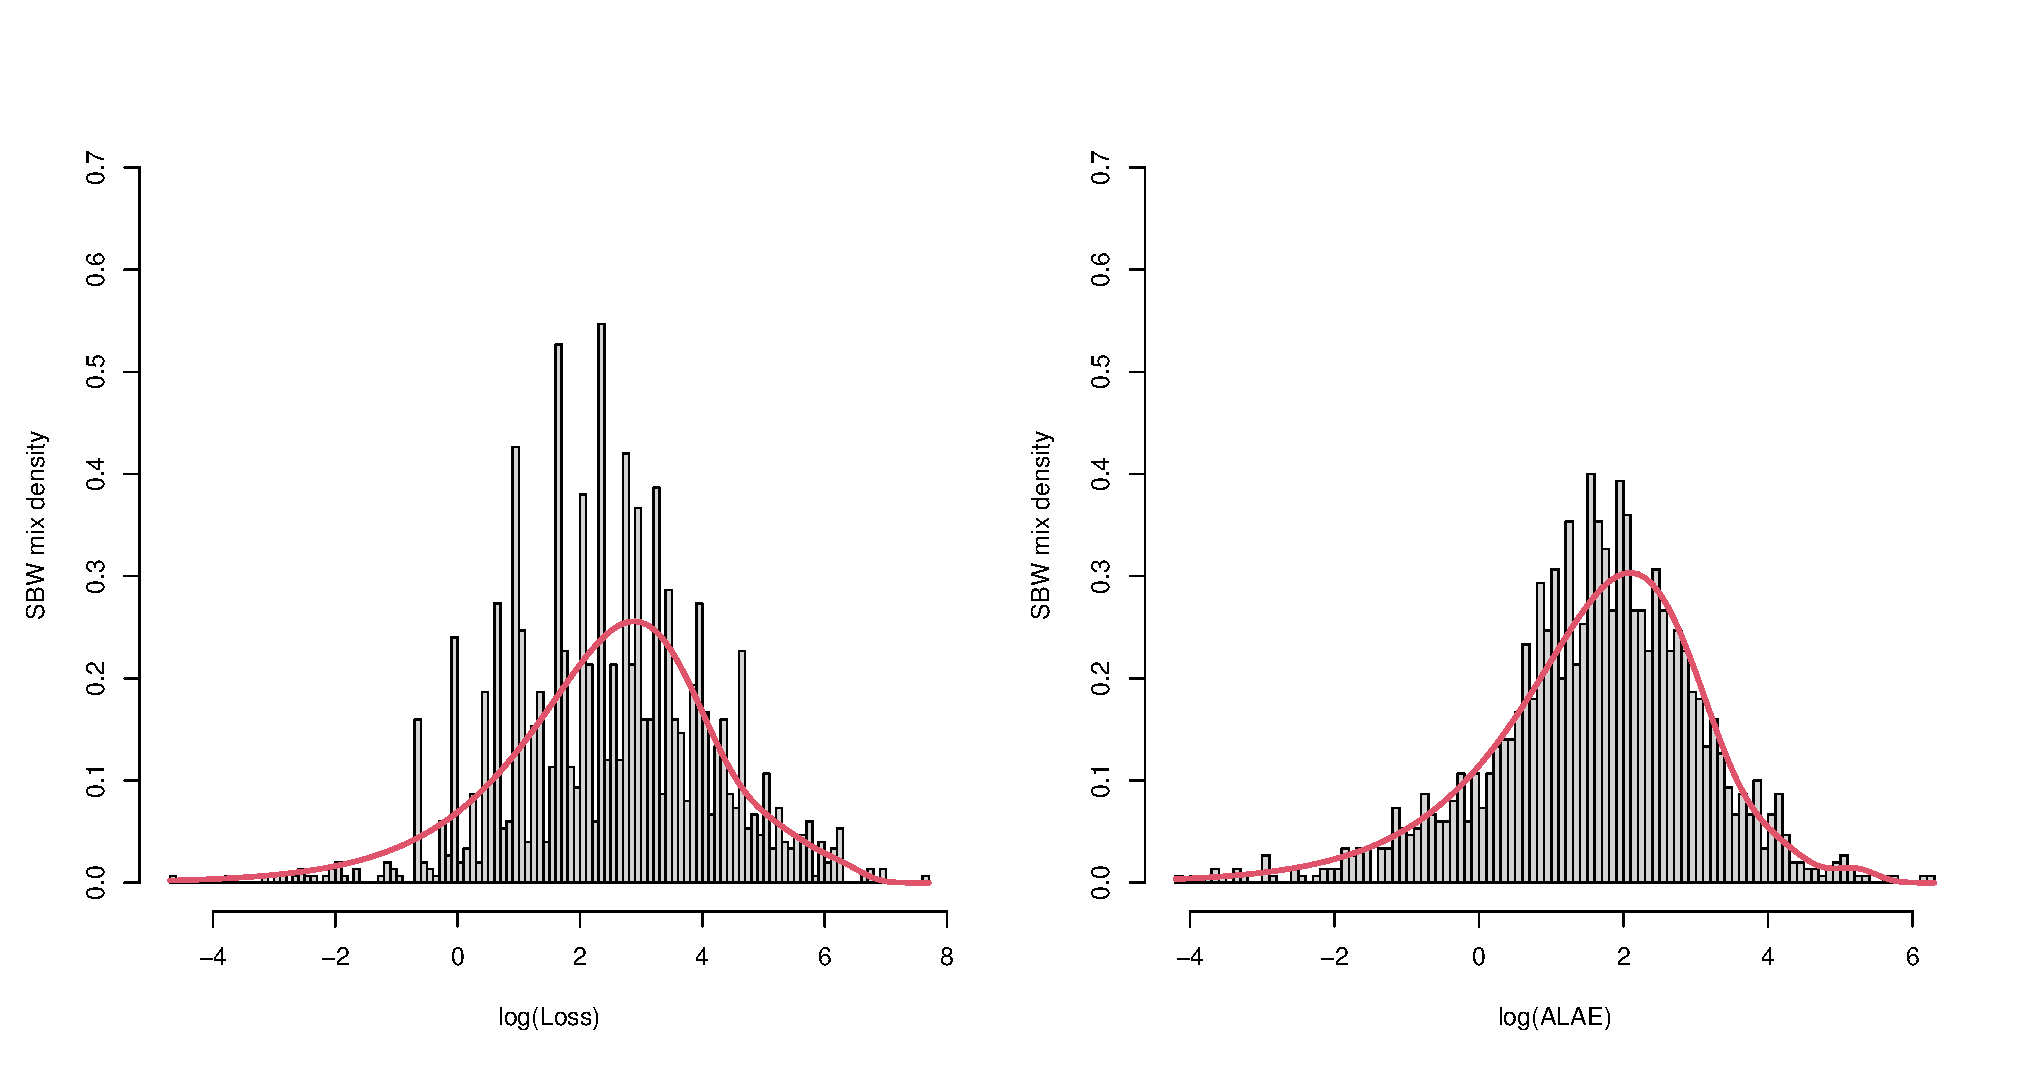
\includegraphics[height=5cm,keepaspectratio=true]{Loss_Alae_SBWMargin_fit.eps}\\
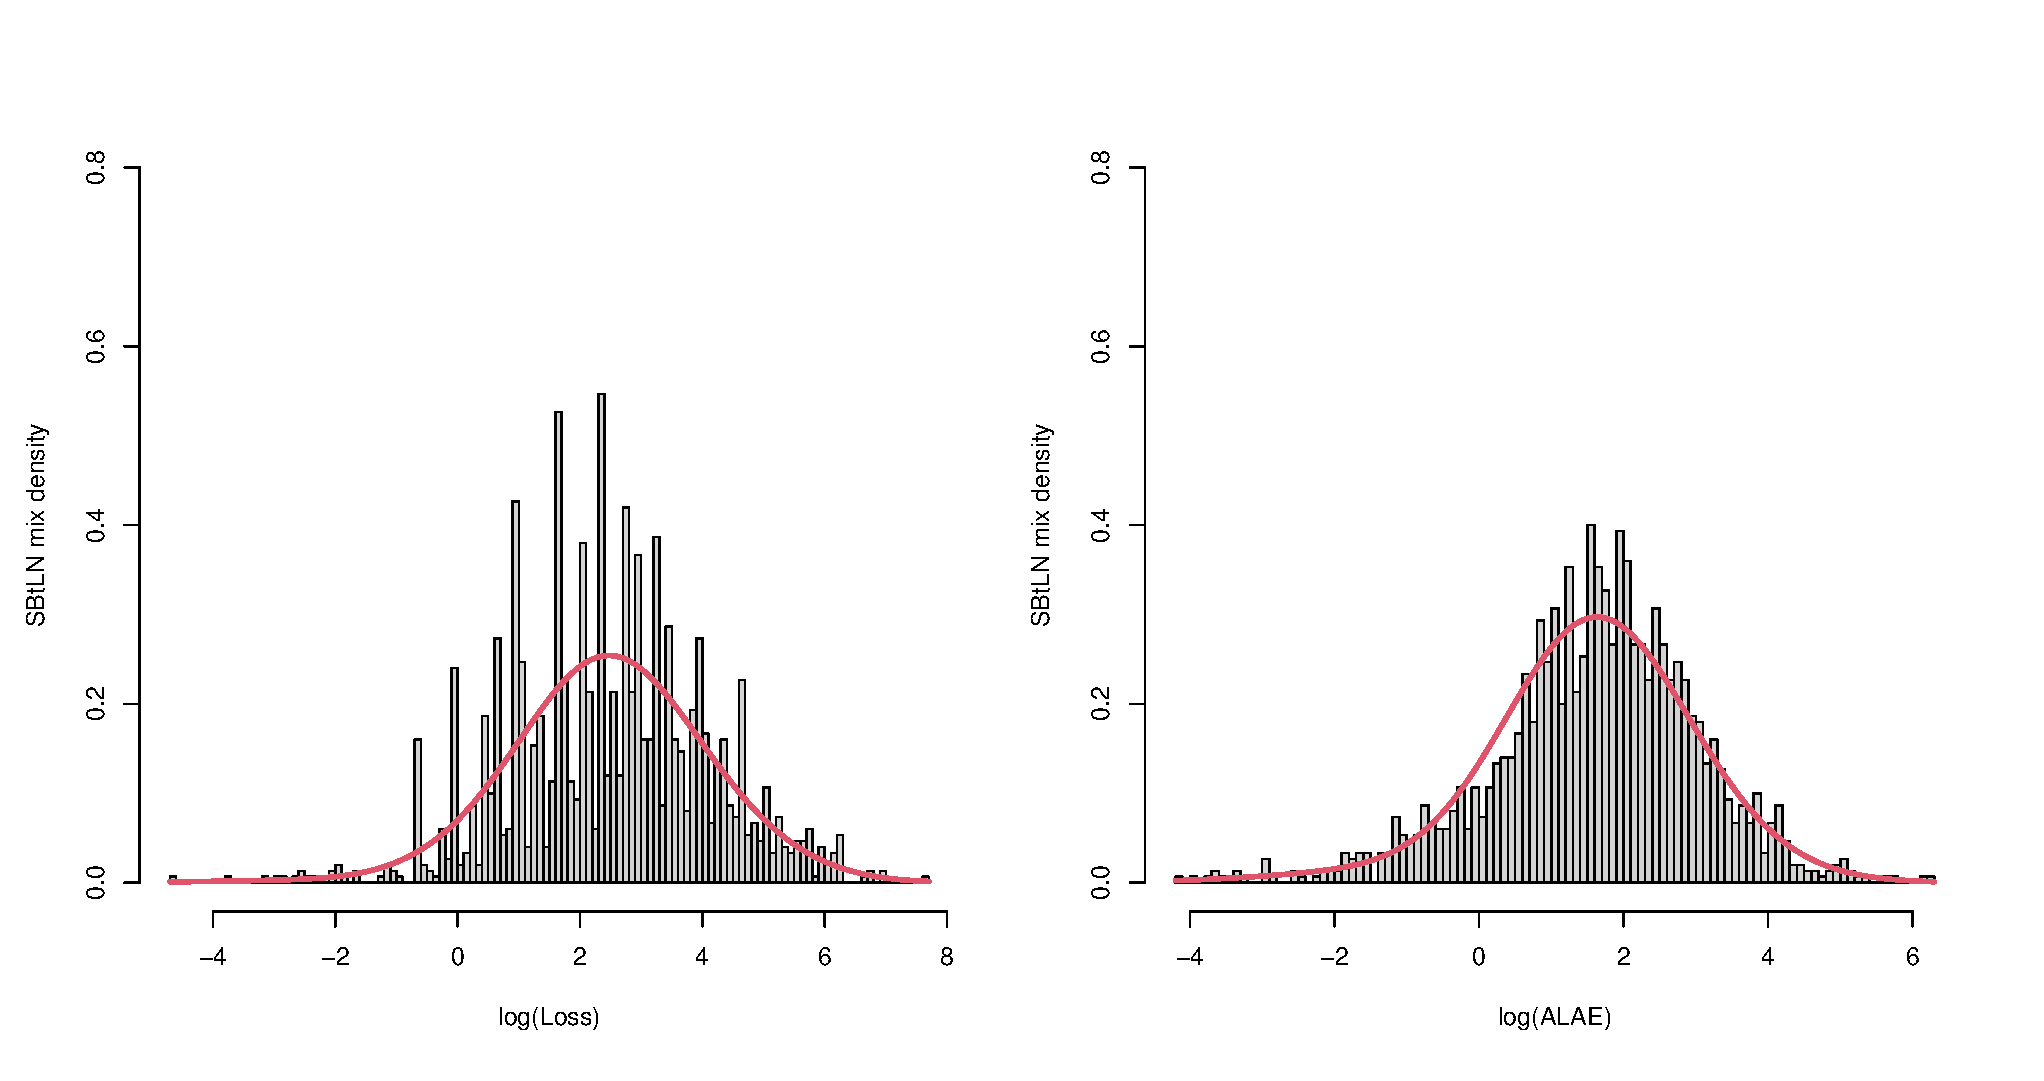
\includegraphics[height=5cm,keepaspectratio=true]{Loss_Alae_SBtlnMargin_fit.eps}
\caption{Density curves of fitted univariate Erlang mixture (top), SBW mixture (middle), and SBtLN mixture (bottom)}
\label{denplots}
\end{figure}

The results of marginal fits are used for the initialization of the penalized EM algorithm in the estimation of the three classes of bivariate size-biased mixture models. A set of the tuning parameter values $\gamma \in \{0, 0.01, 0.02,\ldots, 0.2\}$ has been used to select the best fit model for each model class. Table \ref{tab:BVfits} presents the negative log-likelihood value (NLL), the BIC value, the PEM tuning parameter value, the SB orders of the components, the number of positive component weights, and the model parameter estimates for each model class.

\begin{table}[t]
\scriptsize
\centering
\caption{Fitted bivariate size-biased mixture models}\label{tab:BVfits}
\tabcolsep=4pt
\begin{tabular}{lllllll}
\hline\hline
Model & NLL & BIC & $\gamma$ & SB order & \# pos. weight & Parameter estimate\\
\hline
Erlang & 11489.46 & 23169.06 & 0.13 & \makecell{Loss: 1 -- 8, 13 -- 15, 23, 26, 30, 65 \\ ALAE: 1 -- 3, 6 -- 9, 11, 15, 22, 39} & 25 & $(\hat{\theta}_1,\hat{\theta}_2) = (14.316, 6.566)$ \\
SBW & 11504.06 & 23110.51 & 0.11 & \makecell{Loss: 1, 2, 4, 6, 7, 11 \\ ALAE: 1 -- 5, 8, 13} & 11 & \makecell{$(\hat{\tau}_1, \hat{\tau}_2) = (0.731, 0.822)$\\ $(\hat{\theta}_1, \hat{\theta}_2) = (11.576, 5.382)$} \\
SBtLN & 11487.30 & 23040.42 & 0.15 & \makecell{Loss: 1, 3 -- 7 \\ ALAE: 2 -- 7} & 8 & $(\hat{\sigma}_1, \hat{\sigma}_2) = (1.325, 1.243)$ \\
\hline\hline
\end{tabular}
\end{table}

Amongst the three bivariate SB mixture model classes, the SBtLN mixture model fit gives the smallest BIC value with only eight mixture components fitted by the PEM algorithm at $\gamma = 0.15$. On the other hand, with 25 components, the Erlang mixture model tends to overfit the tail of the data distribution. With 11 components, the fitted SBW model is sparse and the shape parameter estimate $(\hat{\tau}_1, \hat{\tau}_2) = (0.731, 0.822)$ captures the heavy-tailedness of the data. Table \ref{tab_dependence_fit} compares the dependence measures of the fitted bivariate SB mixture models. The result shows that the dependence measures of the fitted Erlang and SBtLN models are lower than those of the SBW model, which may indicate that the fitted SBtLN mixture is overly simplistic while the Erlang mixture is too complex.

\begin{table}[t]
\footnotesize
\centering
\caption{Dependence measures of the fitted bivariate size-biased mixture models}\label{tab_dependence_fit}
\begin{tabular}{ccccc}
\hline\hline
 & Empirical & Erlang & SBW & SBtLN \\
\hline
Spearman's rho & 0.4519 & 0.3025 & 0.3346 & 0.2836 \\
Kendall's tau & 0.3154 & 0.2038 & 0.2273 & 0.1922 \\
\hline\hline
\end{tabular}
\end{table}

Figure \ref{BVdenplots} compares the joint density functions of the fitted bivariate size-biased mixture models and the scatter plots of 3,000 simulated observations from each of the three fitted models. We can see from the density plots that the fitted bivariate Erlang and SBW mixtures render multimodal shapes in the top-right quadrant (Q1) while the BV-SBtLN gives a unimodal curvature. The scatter plots of simulated data contrast the skewness of the fitted models. Even though the BV-SBtLN gives the superior statistical choice globally with a parsimonious eight components, it appears to understate joint upper tail risk that is evident in the empirical data (Figure \ref{scatterplots}).

\begin{figure}[t]
\centering
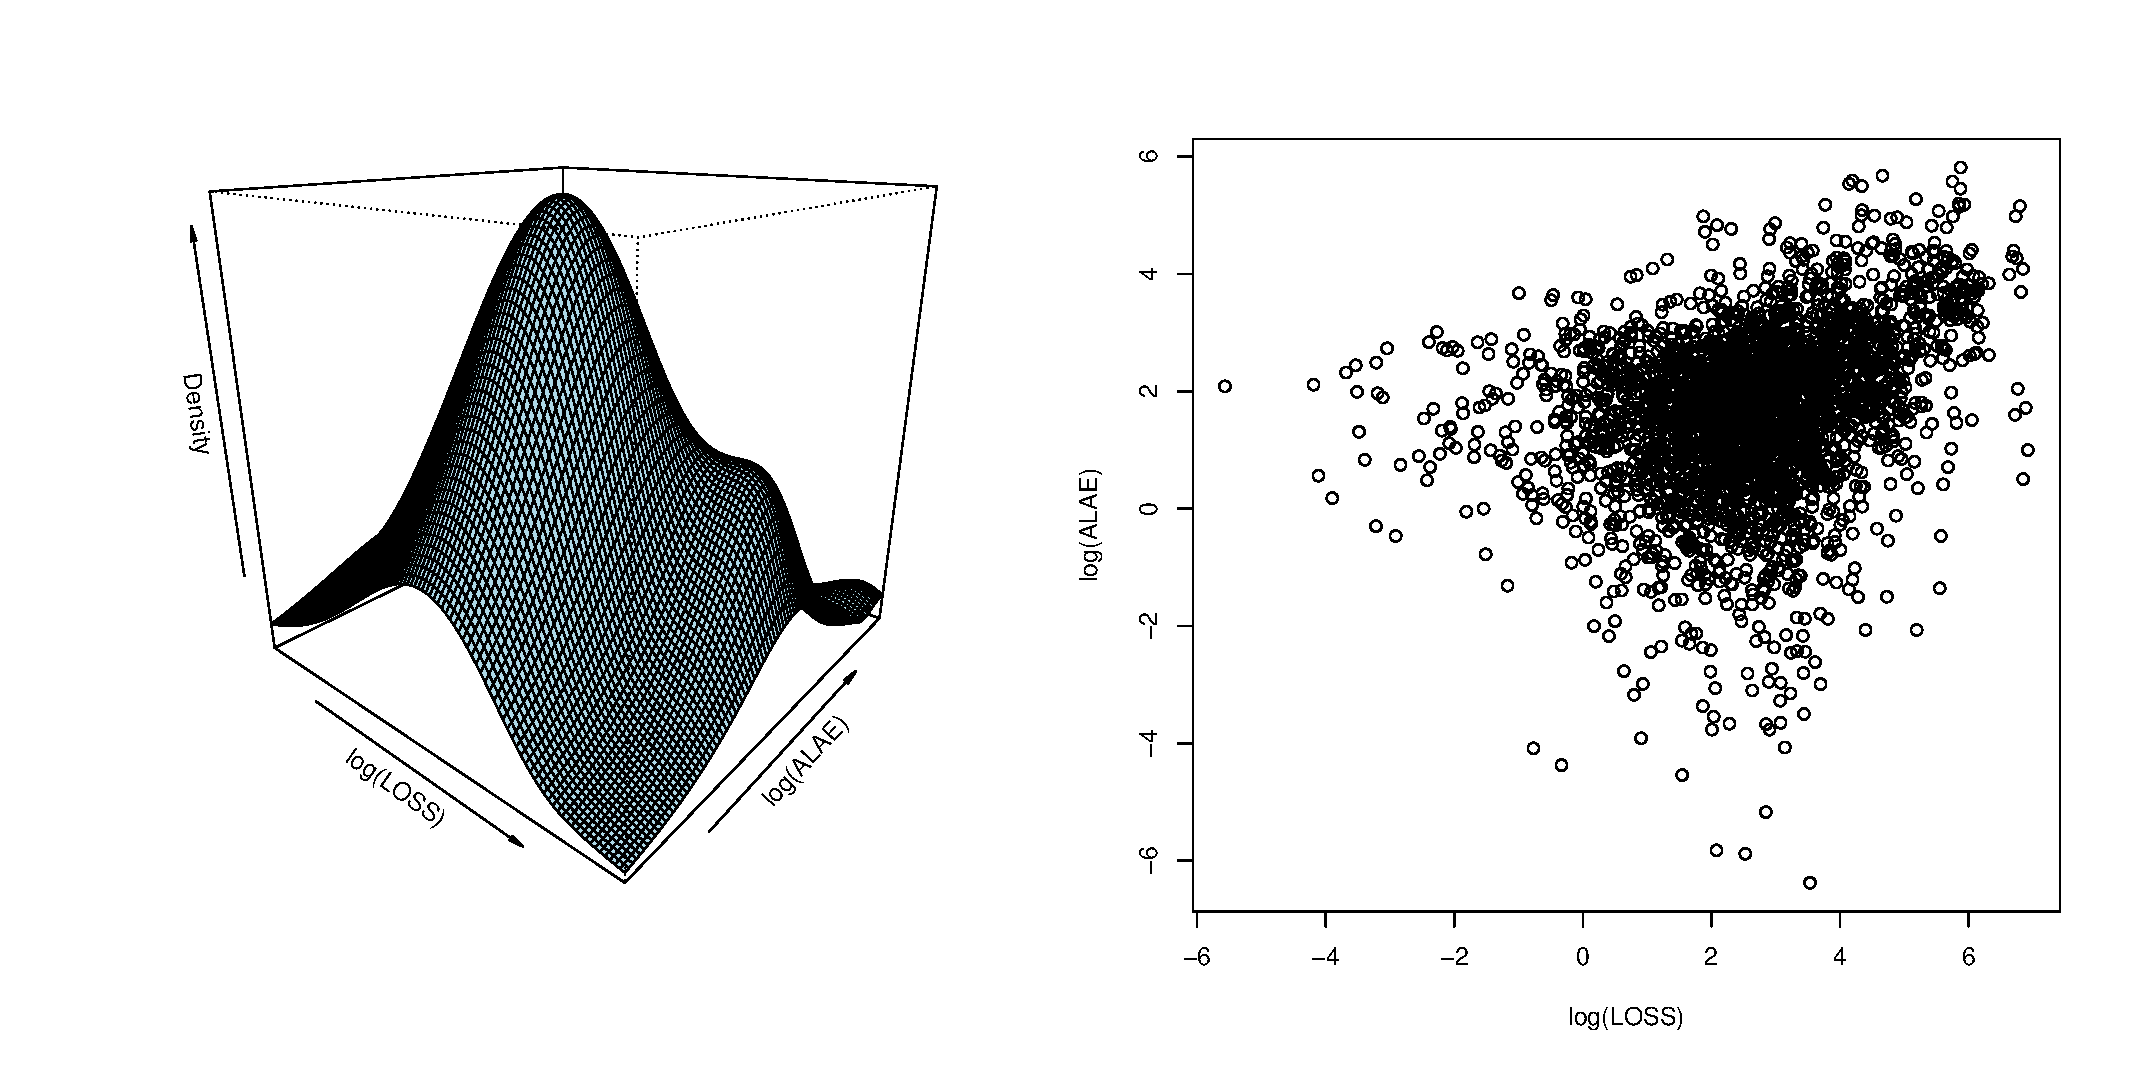
\includegraphics[height=5cm,keepaspectratio=true]{fit3d_BV_Erlang.eps}\\
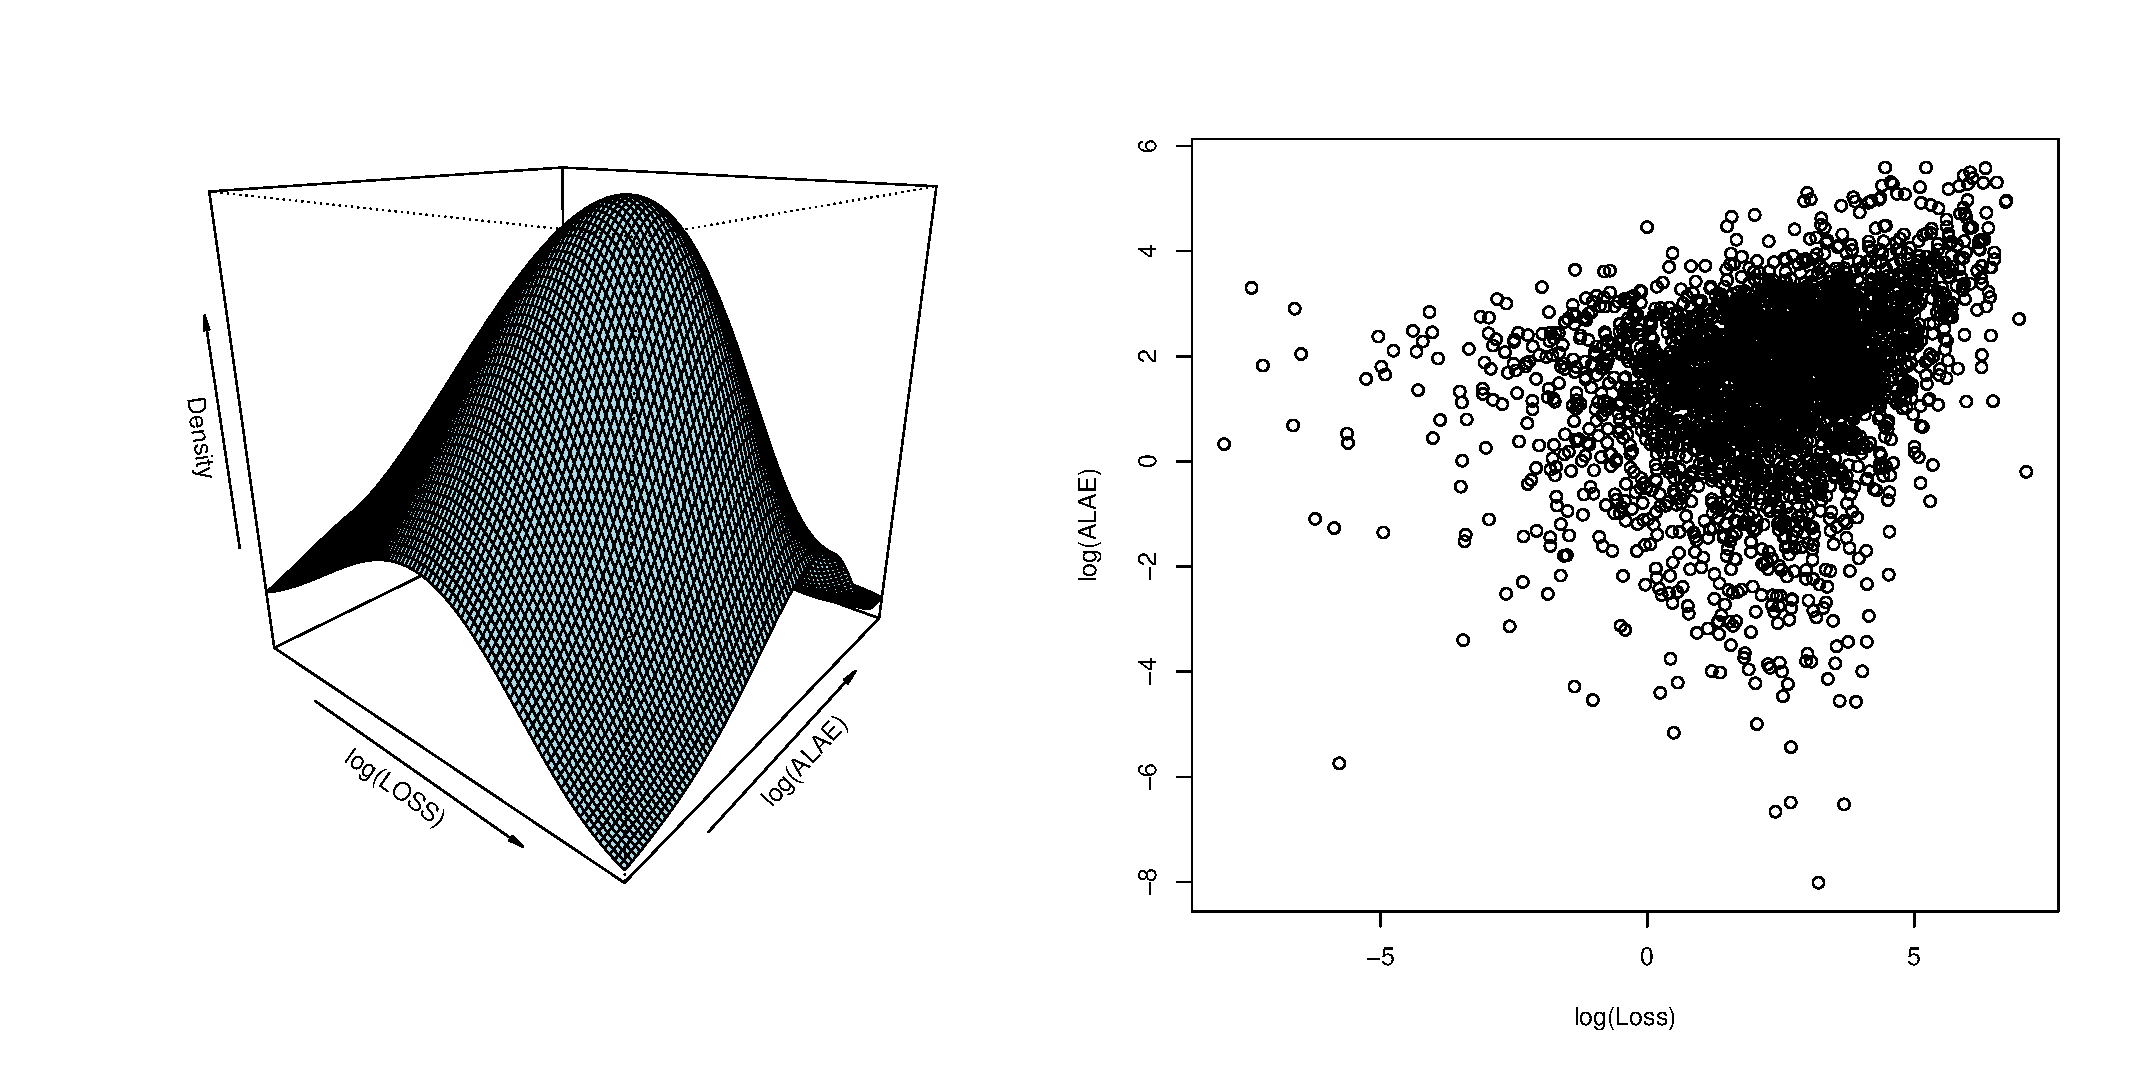
\includegraphics[height=5cm,keepaspectratio=true]{fit3d_BV_SBW.eps}\\
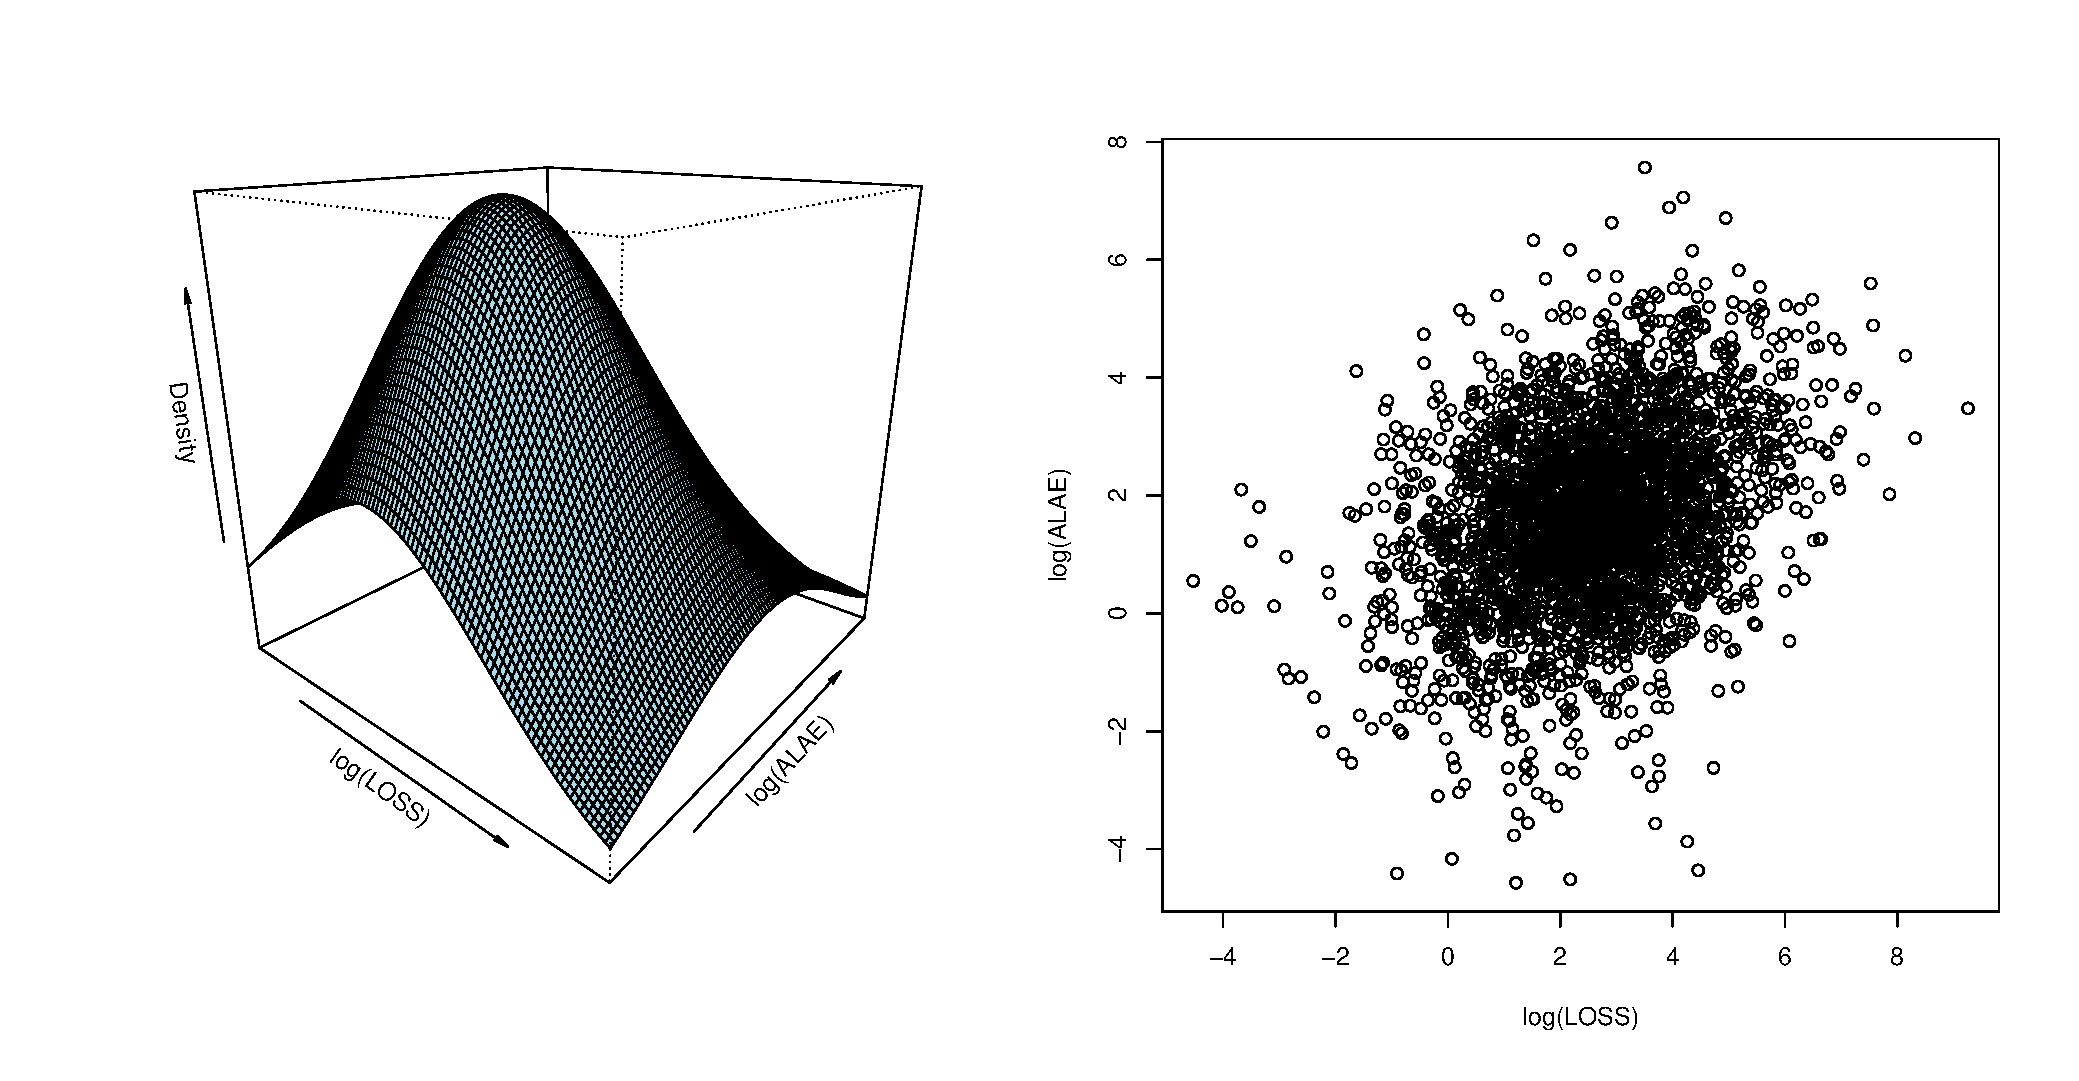
\includegraphics[height=5cm,keepaspectratio=true]{fit3d_BV_SBtLN.eps}
\caption{Joint density curves (left) and scatter plots of 3000 simulated observations (right) from the fitted bivariate Erlang mixture (top), SBW mixture (middle), and SBtLN mixture (bottom) models in log-scale.}
\label{BVdenplots}
\end{figure}

In actuarial science, joint loss modeling is often handled through copulas combined with appropriate marginals \citep{Frees1998, Klugman1999}.

For the purpose of comparison, we fit Clayton, Gumbel, and $t$-copulas with lognormal marginals. Note that the estimation of copula models is performed in two phases in which marginal lognormal models are estimated in the first phase. Then the copula models are fitted in the second phase using the pseudo uniform marginals transformed from the lognormal fits. On the other hand, all model parameters are estimated simultaneously in our approach.

Figure \ref{copulaplots} gives scatter plots of 3000 observations simulated from the three copula fits with lognormal marginals in log-scale. It can be observed from the figure that the Clayton copula incorrectly places all its tight correlation in the lower tail while fanning out loosely in the large claim zone, missing the high-loss dependence. On the other hand, the $t$-copula enforces a symmetric lower-and-upper tail dependence, generating unnecessary joint clustering for small claims. The Gumbel fit gives a strong diagonal spike in the upper-right quadrant, closely mimicking both the log-transformed empirical data from Figure \ref{scatterplots} and the SBW fits in Figure \ref{BVdenplots}.

\begin{figure}[t]
\centering
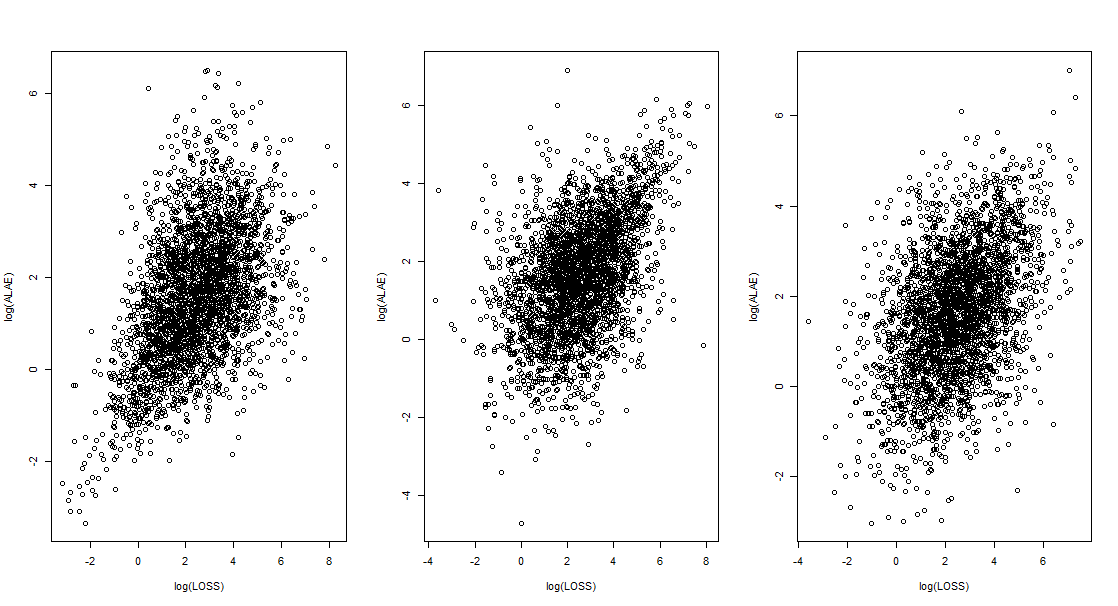
\includegraphics[width=\textwidth,keepaspectratio=true]{copula_fits_lognorm.png}
\caption{Scatter plots of 3000 simulated observations from Clayton copula fit (left), Gumbel copula fit (right), and $t$-copula fit (right) with lognormal marginals in log-scale.}
\label{copulaplots}
\end{figure}


\section{Conclusion}\label{sec6}
In this paper, we have extended the univariate size-biased mixture framework to a multivariate setting, providing an effective tool for modeling complex, dependent loss data structures. By leveraging the weak-denseness property of SB mixtures, specifically Erlang, size-biased Weibull, and size-biased truncated lognormal mixture distributions, we demonstrated that these models can approximate a wide range of multivariate continuous distributions with high precision.

A key contribution of this research is the implementation of a Penalized EM (PEM) algorithm for parameter estimation. This approach effectively addresses the common issue of overfitting inherent in classical EM algorithms by purging statistically insignificant components. As demonstrated in our numerical examples, the PEM algorithm results in more parsimonious and interpretable models without sacrificing significant goodness-of-fit.

The application to a bivariate insurance liability dataset (Loss and ALAE) highlighted the practical utility of our proposed models. Our analysis revealed that while the Erlang mixture provides a flexible fit, it tends toward over-complexity with a high number of components. In contrast, the SBtLN mixture model offered the most efficient fit in terms of the Bayesian Information Criterion (BIC), while the SBW mixture proved effective in capturing the heavy-tailed dependence structures often found in insurance data.

Overall, the multivariate size-biased mixture models, supported by penalized estimation, offers a powerful and flexible addition to the statistical toolkit for actuaries and data scientists working with heterogeneous, dependent populations.

Future research could explore the extension of this framework to include covariate effects through mixture-of-experts models \citep{fung2019class_theory, tseung2021lrmoe, fung2025mixture} or investigate the performance of these multivariate SB mixtures in higher-dimensional data. The lack of upper tail dependence poses a limitation of the proposed multivariate model. This issue is expected to be overcome by introducing shared latent model parameters. We will pursue this approach in the future.


%% ==================================================================
%% Appendix (kept inside a group, as in the CSAM template, so that the
%% redefinition of \section does not affect the reference list)
%% ==================================================================
{\appendix
\renewcommand{\theequation}{\thesection.\arabic{equation}}

\section{Proofs of Propositions 1--3}\label{app:props}

From the definition (\ref{sb_den})
\begin{equation*}
g(x;s,\theta) =\frac{x^{s-1}h(x;\theta)}{\mu(s-1;\theta)},
\end{equation*}
we obtain, for every $r$ for which the moment exists,
\begin{equation}\label{A1}
\int_0^\infty x^r g(x;s,\theta)\,dx
= \frac{1}{\mu(s-1;\theta)} \int_0^\infty x^{r+s-1}h(x;\theta)\,dx
= \frac{\mu(s+r-1;\theta)}{\mu(s-1;\theta)}.
\end{equation}

\subsection*{Proof of Proposition \ref{prop:cov}}

For the bivariate density
\begin{equation*}
f_{u,v}(x,y) = \sum_{l=1}^{M_u}\sum_{m=1}^{M_v} \alpha^{(u,v)}_{lm} g(x;s_l^{(u)},\theta_u) g(y;s_m^{(v)},\theta_v),
\end{equation*}
the covariance is
\begin{equation*}
\operatorname{Cov}(X_u,X_v) = \sum_{l=1}^{M_u}\sum_{m=1}^{M_v} \left( \alpha^{(u,v)}_{lm} -\alpha_l^{(u)}\alpha_m^{(v)} \right) m(s_l^{(u)},\theta_u)m(s_m^{(v)},\theta_v).
\end{equation*}

\begin{proof}
By the mixture representation and Tonelli's theorem,
\begin{align*}
\mathbb E[X_uX_v] &= \int_0^\infty\int_0^\infty xy\,f_{u,v}(x,y)\,dx\,dy\\
&= \sum_{l=1}^{M_u}\sum_{m=1}^{M_v} \alpha^{(u,v)}_{lm} \left[ \int_0^\infty xg(x;s_l^{(u)},\theta_u)\,dx \right] \left[ \int_0^\infty yg(y;s_m^{(v)},\theta_v)\,dy \right].
\end{align*}
Then
\begin{equation}\label{A2}
\mathbb E[X_uX_v] = \sum_{l,m} \alpha^{(u,v)}_{lm} \frac{\mu(s_l^{(u)};\theta_u)}{\mu(s_l^{(u)}-1;\theta_u)} \frac{\mu(s_m^{(v)};\theta_v)}{\mu(s_m^{(v)}-1;\theta_v)}.
\end{equation}
The marginal mixing probabilities are
\begin{equation*}
\alpha_l^{(u)} = \sum_m\alpha_{lm}^{(u,v)}, \qquad \alpha_m^{(v)} = \sum_l\alpha_{lm}^{(u,v)}.
\end{equation*}
Therefore,
\begin{equation*}
\mathbb E[X_u] = \sum_l\alpha_l^{(u)}m(s_l^{(u)},\theta_u), \qquad \mathbb E[X_v] = \sum_m\alpha_m^{(v)}m(s_m^{(v)},\theta_v).
\end{equation*}
Consequently,
\begin{equation}\label{A3}
\mathbb E[X_u]\mathbb E[X_v] = \sum_l\sum_m \alpha_l^{(u)}\alpha_m^{(v)} m(s_l^{(u)},\theta_u)m(s_m^{(v)},\theta_v).
\end{equation}
Subtracting (\ref{A3}) from (\ref{A2}) gives
\begin{equation*}
\operatorname{Cov}(X_u,X_v) = \sum_{l,m} \left( \alpha^{(u,v)}_{lm} -\alpha_l^{(u)}\alpha_m^{(v)} \right) m(s_l^{(u)},\theta_u)m(s_m^{(v)},\theta_v).
\end{equation*}
This proves Proposition \ref{prop:cov}.
\end{proof}

\subsection*{Proof of Proposition \ref{prop:rho}}

Let
\begin{equation*}
F_u(x) = \sum_{l'=1}^{M_u}\alpha_{l'}^{(u)} G(x;s_{l'}^{(u)},\theta_u) \quad\text{and}\quad F_v(y)=\sum_{m'=1}^{M_v}\alpha_{m'}^{(v)} G(y;s_{m'}^{(v)},\theta_v)
\end{equation*}
be the marginal distribution functions. Then Spearman's rho is
\begin{equation*}
\rho = 12 \sum_{l,m,l',m'} \alpha^{(u,v)}_{lm} \alpha_{l'}^{(u)} \alpha_{m'}^{(v)} \lambda(s_l^{(u)},s_{l'}^{(u)},\theta_u) \lambda(s_m^{(v)},s_{m'}^{(v)},\theta_v) -3,
\end{equation*}
where
\begin{equation*}
\lambda(s,t,\theta) = \int_0^\infty G(x;s,\theta)g(x;t,\theta)\,dx.
\end{equation*}

\begin{proof}
For continuous random variables,
\begin{equation*}
U_u=F_u(X_u),\qquad U_v=F_v(X_v)
\end{equation*}
are uniform on $(0,1)$. Hence
\begin{equation*}
\mathbb E[U_u]=\mathbb E[U_v]=\frac12, \qquad \operatorname{Var}(U_u)=\operatorname{Var}(U_v)=\frac1{12},
\end{equation*}
and thus
\begin{equation}\label{A4}
\rho = 12\,\mathbb E[F_u(X_u)F_v(X_v)]-3.
\end{equation}
Using the bivariate mixture density,
\begin{equation*}
\mathbb E[F_u(X_u)F_v(X_v)] = \sum_{l,m}\alpha^{(u,v)}_{lm} \int_0^\infty\int_0^\infty F_u(x)F_v(y) \, g(x;s_l^{(u)},\theta_u) g(y;s_m^{(v)},\theta_v)\,dx\,dy.
\end{equation*}
Since the integrand separates in $x$ and $y$,
\begin{equation}\label{A5}
\mathbb E[F_u(X_u)F_v(X_v)] = \sum_{l,m}\alpha^{(u,v)}_{lm} \left[ \int_0^\infty F_u(x)g(x;s_l^{(u)},\theta_u)\,dx \right] \left[ \int_0^\infty F_v(y)g(y;s_m^{(v)},\theta_v)\,dy \right].
\end{equation}
Now expand the marginal cdfs:
\begin{equation*}
F_u(x) = \sum_{l'}\alpha_{l'}^{(u)} G(x;s_{l'}^{(u)},\theta_u).
\end{equation*}
Therefore,
\begin{equation*}
\int_0^\infty F_u(x)g(x;s_l^{(u)},\theta_u)\,dx = \sum_{l'}\alpha_{l'}^{(u)} \int_0^\infty G(x;s_{l'}^{(u)},\theta_u) g(x;s_l^{(u)},\theta_u)\,dx.
\end{equation*}
Thus,
\begin{equation}\label{A6}
\int_0^\infty F_u(x)g(x;s_l^{(u)},\theta_u)\,dx = \sum_{l'}\alpha_{l'}^{(u)} \lambda(s_{l'}^{(u)},s_l^{(u)},\theta_u).
\end{equation}
Similarly,
\begin{equation}\label{A7}
\int_0^\infty F_v(y)g(y;s_m^{(v)},\theta_v)\,dy = \sum_{m'}\alpha_{m'}^{(v)}\lambda(s_{m'}^{(v)},s_m^{(v)},\theta_v).
\end{equation}
Substituting (\ref{A6}) and (\ref{A7}) into (\ref{A5}), and then into (\ref{A4}), yields
\begin{equation*}
\rho = 12 \sum_{l,m,l',m'} \alpha^{(u,v)}_{lm} \alpha_{l'}^{(u)} \alpha_{m'}^{(v)} \lambda(s_{l'}^{(u)},s_l^{(u)},\theta_u) \lambda(s_{m'}^{(v)},s_m^{(v)},\theta_v) -3.
\end{equation*}
This proves Proposition \ref{prop:rho}.
\end{proof}

\subsection*{Proof of Proposition \ref{prop:tau}}

Kendall's tau is
\begin{equation*}
\tau = 4 \sum_{l,m,l',m'} \alpha^{(u,v)}_{lm} \alpha^{(u,v)}_{l'm'} \lambda(s_l^{(u)},s_{l'}^{(u)},\theta_u) \lambda(s_m^{(v)},s_{m'}^{(v)},\theta_v) -1.
\end{equation*}

\begin{proof}
Let $(X_u,X_v)$ and $(X_u',X_v')$ be independent and identically distributed copies of the bivariate size-biased mixture vector. For continuous random variables,
\begin{equation}\label{A8}
\tau = 4\,\mathbb E\left[ F_{u,v}(X_u,X_v) \right]-1,
\end{equation}
where
\begin{equation*}
F_{u,v}(x,y) = \Pr(X_u\le x,X_v\le y).
\end{equation*}
The joint cdf is
\begin{equation}\label{A9}
F_{u,v}(x,y) = \sum_{l',m'} \alpha_{l'm'}^{(u,v)} G(x;s_{l'}^{(u)},\theta_u) G(y;s_{m'}^{(v)},\theta_v),
\end{equation}
because each component has independent coordinates. Using the mixture representation of $(X_u,X_v)$,
\begin{equation*}
\mathbb E[F_{u,v}(X_u,X_v)] = \sum_{l,m}\alpha_{lm}^{(u,v)} \int_0^\infty\int_0^\infty F_{u,v}(x,y)\, g(x;s_l^{(u)},\theta_u) g(y;s_m^{(v)},\theta_v)\,dx\,dy.
\end{equation*}
Substitute (\ref{A9}):
\begin{multline*}
\mathbb E[F_{u,v}(X_u,X_v)] = \sum_{l,m}\sum_{l',m'} \alpha_{lm}^{(u,v)}\alpha_{l'm'}^{(u,v)} \int_0^\infty G(x;s_{l'}^{(u)},\theta_u) g(x;s_l^{(u)},\theta_u)\,dx\\
\times \int_0^\infty G(y;s_{m'}^{(v)},\theta_v) g(y;s_m^{(v)},\theta_v)\,dy.
\end{multline*}
By the definition of $\lambda$ function,
\begin{equation*}
\mathbb E[F_{u,v}(X_u,X_v)] =\sum_{l,m,l',m'} \alpha_{lm}^{(u,v)}\alpha_{l'm'}^{(u,v)} \lambda(s_{l'}^{(u)},s_l^{(u)},\theta_u) \lambda(s_{m'}^{(v)},s_m^{(v)},\theta_v).
\end{equation*}
Substitution into (\ref{A8}) gives
\begin{equation*}
\tau = 4 \sum_{l,m,l',m'} \alpha_{lm}^{(u,v)}\alpha_{l'm'}^{(u,v)} \lambda(s_l^{(u)},s_{l'}^{(u)},\theta_u) \lambda(s_m^{(v)},s_{m'}^{(v)},\theta_v) -1.
\end{equation*}
Hence Proposition \ref{prop:tau} follows.
\end{proof}


\section{Proof of upper tail independence}\label{app:tail}

Let
\begin{equation*}
\bar G_{k,s}(x):=1-G(x;s,\theta_k) =\int_x^\infty g(y;s,\theta_k)\,dy
\end{equation*}
denote the survival function of a size-biased component in coordinate $k$, where
\begin{equation*}
g(y;s,\theta_k)=\frac{y^{s-1}h(y;\theta_k)}{\mu(s-1;\theta_k)}.
\end{equation*}
We prove that the upper-tail dependence coefficient
\begin{equation*}
\lambda_U =\lim_{q\to1} \Pr\left(X_u>F_u^{-1}(q)\mid X_v>F_v^{-1}(q)\right)
\end{equation*}
is zero.

\begin{proof}
Set
\begin{equation*}
x_q=F_u^{-1}(q),\qquad y_q=F_v^{-1}(q).
\end{equation*}
Since $F_u(x_q)=F_v(y_q)=q$,
\begin{equation*}
\Pr(X_u>x_q)=\Pr(X_v>y_q)=1-q.
\end{equation*}
The joint survival function associated with (\ref{pair_density}) is
\begin{equation*}
\Pr(X_u>x,X_v>y) = \sum_{l=1}^{M_u}\sum_{m=1}^{M_v} \alpha^{(u,v)}_{l,m} \bar G_{u,s_l^{(u)}}(x) \bar G_{v,s_m^{(v)}}(y),
\end{equation*}
because the coordinates are conditionally independent within each mixture component. Hence
\begin{equation*}
\lambda_U = \lim_{q\to1} \frac{ \sum_{l,m}\alpha^{(u,v)}_{l,m} \bar G_{u,s_l^{(u)}}(x_q) \bar G_{v,s_m^{(v)}}(y_q) }{1-q}.
\end{equation*}
We now use the ordering of the size-biased components. If $s<t$, then
\begin{equation*}
\bar G_{k,s}(x) = \frac{1}{\mu(s-1;\theta_k)} \int_x^\infty z^{s-1}h(z;\theta_k)\,dz
\end{equation*}
and, for $z\ge x$,
\begin{equation*}
z^{s-1} =z^{t-1}z^{s-t} \le x^{s-t}z^{t-1}.
\end{equation*}
Therefore,
\begin{equation*}
\bar G_{k,s}(x) \le \frac{\mu(t-1;\theta_k)}{\mu(s-1;\theta_k)} x^{s-t}\bar G_{k,t}(x).
\end{equation*}
Since $s-t<0$, it follows that
\begin{equation*}
\frac{\bar G_{k,s}(x)}{\bar G_{k,t}(x)} \longrightarrow 0 \qquad (x\to\infty).
\end{equation*}
Thus, among the finitely many size-biased components, the component with the largest order dominates the upper tail. In particular, for every $(l,m)$, there are finite constants $(C_{u,l},C_{v,m})$ such that, for sufficiently large $(x,y)$,
\begin{equation*}
\bar G_{u,s_l^{(u)}}(x)\le C_{u,l}\bar F_u(x), \qquad \bar G_{v,s_m^{(v)}}(y)\le C_{v,m}\bar F_v(y),
\end{equation*}
where
\begin{equation*}
\bar F_u(x)=1-F_u(x),\qquad \bar F_v(y)=1-F_v(y).
\end{equation*}
Consequently,
\begin{align*}
\Pr(X_u>x_q,X_v>y_q) &\le \sum_{l,m}\alpha^{(u,v)}_{l,m} C_{u,l}C_{v,m} \bar F_u(x_q)\bar F_v(y_q)\\
&=C(1-q)^2
\end{align*}
for some finite constant $C$. Dividing by $\Pr(X_v>y_q)= 1-q$ gives
\begin{equation*}
\Pr(X_u>x_q\mid X_v>y_q) \le C(1-q)\longrightarrow 0.
\end{equation*}
Therefore, $\lambda_U=0$. Hence any pair of random variables from the bivariate size-biased mixture is asymptotically independent in the upper tail even though dependence can still arise at finite levels through the joint mixture weights $\alpha^{(u,v)}_{l,m}$.
\end{proof}
}


%% ==================================================================
%% References (CSAM style; entries mirror references.bib)
%% ==================================================================
\begin{reference}
\bibitem[Ahn et~al.(2026)Ahn, Jeong, and Oh]{ahn2026normal}
Ahn JY, Jeong H, and Oh R (2026). A Normal-Gamma copula for dependence modeling in collective risk models, {\em ASTIN Bulletin: The Journal of the IAA}, {\bf 56}, 1066--1090.

\bibitem[Aradhye et~al.(2024a)Aradhye, Tzougas, and Bhati]{aradhye2024copula}
Aradhye G, Tzougas G, and Bhati D (2024a). A copula-based bivariate composite model for modelling claim costs, {\em Mathematics}, {\bf 12}, 350.

\bibitem[Aradhye et~al.(2024b)Aradhye, Tzougas, and Bhati]{aradhye2024em}
Aradhye G, Tzougas G, and Bhati D (2024b). EM estimation for the mixed Pareto regression model for claim severities, {\em Communications in Statistics - Theory and Methods}, {\bf 53}, 5507--5523.

\bibitem[Bae and Ko(2020)]{bae2020mixtures}
Bae T and Ko B (2020). On the mixtures of length-biased Weibull distributions for loss severity modeling, {\em Journal of the Korean Statistical Society}, {\bf 49}, 422--438.

\bibitem[Bae and Miljkovic(2024)]{bae2024loss}
Bae T and Miljkovic T (2024). Loss modeling with the size-biased lognormal mixture and the entropy regularized EM algorithm, {\em Insurance: Mathematics and Economics}, {\bf 117}, 182--195.

\bibitem[Blostein and Miljkovic(2019)]{blostein2019modeling}
Blostein M and Miljkovic T (2019). On modeling left-truncated loss data using mixtures of distributions, {\em Insurance: Mathematics and Economics}, {\bf 85}, 35--46.

\bibitem[Bouguila and Fan(2020)]{Bouguila2020}
Bouguila N and Fan W (2020). {\em Mixture Models and Applications}, Springer.

\bibitem[Chen et~al.(2022)Chen, Dassios, and Tzougas]{chen2022em}
Chen Z, Dassios A, and Tzougas G (2022). EM estimation for the bivariate mixed exponential regression model, {\em Risks}, {\bf 10}, 105.

\bibitem[Dempster et~al.(1977)Dempster, Laird, and Rubin]{dempster1977maximum}
Dempster AP, Laird NM, and Rubin DB (1977). Maximum likelihood from incomplete data via the EM algorithm, {\em Journal of the Royal Statistical Society: Series B (Methodological)}, {\bf 39}, 1--22.

\bibitem[Figueiredo and Jain(2002)]{Figueiredo}
Figueiredo MAT and Jain AK (2002). Unsupervised learning of finite mixture models, {\em IEEE Transactions on Pattern Analysis and Machine Intelligence}, {\bf 24}, 381--396.

\bibitem[Frees and Valdez(1998)]{Frees1998}
Frees EW and Valdez EA (1998). Understanding relationships using copulas, {\em North American Actuarial Journal}, {\bf 2}, 1--25.

\bibitem[Fung(2022)]{fung2022maximum}
Fung TC (2022). Maximum weighted likelihood estimator for robust heavy-tail modelling of finite mixture models, {\em Insurance: Mathematics and Economics}, {\bf 107}, 180--198.

\bibitem[Fung et~al.(2019a)Fung, Badescu, and Lin]{fung2019class_freq}
Fung TC, Badescu AL, and Lin XS (2019a). A class of mixture of experts models for general insurance: Application to correlated claim frequencies, {\em ASTIN Bulletin: The Journal of the IAA}, {\bf 49}, 647--688.

\bibitem[Fung et~al.(2019b)Fung, Badescu, and Lin]{fung2019class_theory}
Fung TC, Badescu AL, and Lin XS (2019b). A class of mixture of experts models for general insurance: Theoretical developments, {\em Insurance: Mathematics and Economics}, {\bf 89}, 111--127.

\bibitem[Fung et~al.(2021)Fung, Badescu, and Lin]{fung2021new}
Fung TC, Badescu AL, and Lin XS (2021). A new class of severity regression models with an application to IBNR prediction, {\em North American Actuarial Journal}, {\bf 25}, 206--231.

\bibitem[Fung et~al.(2022)Fung, Badescu, and Lin]{fung2022fitting}
Fung TC, Badescu AL, and Lin XS (2022). Fitting censored and truncated regression data using the mixture of experts models, {\em North American Actuarial Journal}, {\bf 26}, 496--520.

\bibitem[Fung et~al.(2024)Fung, Jeong, and Tzougas]{fung2024soft}
Fung TC, Jeong H, and Tzougas G (2024). Soft splicing model: Bridging the gap between composite model and finite mixture model, {\em Scandinavian Actuarial Journal}, {\bf 2024}, 168--197.

\bibitem[Fung and Tseung(2025)]{fung2025mixture}
Fung TC and Tseung SC (2025). Mixture of experts models for multilevel data: Modeling framework and approximation theory, {\em Neurocomputing}, {\bf 626}, 129357.

\bibitem[Fung et~al.(2023)Fung, Tzougas, and W\"uthrich]{fung2023mixture}
Fung TC, Tzougas G, and W\"uthrich MV (2023). Mixture composite regression models with multi-type feature selection, {\em North American Actuarial Journal}, {\bf 27}, 396--428.

\bibitem[Gupta and Kirmani(1990)]{gupta1990role}
Gupta RC and Kirmani SNUA (1990). The role of weighted distributions in stochastic modeling, {\em Communications in Statistics - Theory and Methods}, {\bf 19}, 3147--3162.

\bibitem[Jeong et~al.(2021)Jeong, Chang, and Valdez]{jeong2021nonconvex}
Jeong H, Chang H, and Valdez EA (2021). A non-convex regularization approach for stable estimation of loss development factors, {\em Scandinavian Actuarial Journal}, {\bf 2021}, 779--803.

\bibitem[Jeong and Dey(2020)]{jeong2020application}
Jeong H and Dey DK (2020). Application of vine copula for multi-line insurance reserving, {\em Risks}, {\bf 8}, 111.

\bibitem[Jeong et~al.(2023)Jeong, Tzougas, and Fung]{jeong2023multivariate}
Jeong H, Tzougas G, and Fung TC (2023). Multivariate claim count regression model with varying dispersion and dependence parameters, {\em Journal of the Royal Statistical Society Series A: Statistics in Society}, {\bf 186}, 61--83.

\bibitem[Jeong and Valdez(2020)]{jeong2020predictive}
Jeong H and Valdez EA (2020). Predictive compound risk models with dependence, {\em Insurance: Mathematics and Economics}, {\bf 94}, 182--195.

\bibitem[Klugman et~al.(2019)Klugman, Panjer, and Willmot]{Klugman2019}
Klugman SA, Panjer HH, and Willmot GE (2019). {\em Loss Models: From Data to Decisions} (5th ed), John Wiley \& Sons, Hoboken.

\bibitem[Klugman and Parsa(1999)]{Klugman1999}
Klugman SA and Parsa R (1999). Fitting bivariate loss distributions with copulas, {\em Insurance: Mathematics and Economics}, {\bf 24}, 139--148.

\bibitem[Lee and Lin(2010)]{leelin2010}
Lee SCK and Lin XS (2010). Modeling and evaluating insurance losses via mixtures of Erlang distributions, {\em North American Actuarial Journal}, {\bf 14}, 107--130.

\bibitem[Lee and Lin(2012)]{leelin2012}
Lee SCK and Lin XS (2012). Modeling dependent risks with multivariate Erlang mixtures, {\em ASTIN Bulletin: The Journal of the IAA}, {\bf 42}, 153--180.

\bibitem[Lindsay(1995)]{Lindsay1995}
Lindsay BG (1995). {\em Mixture Models: Theory, Geometry and Applications}, NSF-CBMS Regional Conference Series in Probability and Statistics, {\bf 5}, Institute of Mathematical Statistics, Hayward.

\bibitem[Patil and Rao(1978)]{patil:1978}
Patil GP and Rao CR (1978). Weighted distributions and size-biased sampling with applications to wildlife populations and human families, {\em Biometrics}, {\bf 34}, 179--189.

\bibitem[Titterington et~al.(1985)Titterington, Smith, and Makov]{Titterington1985}
Titterington DM, Smith AFM, and Makov UE (1985). {\em Statistical Analysis of Finite Mixture Distributions}, John Wiley \& Sons, Chichester.

\bibitem[Tseung et~al.(2021)Tseung, Badescu, Fung, and Lin]{tseung2021lrmoe}
Tseung SC, Badescu AL, Fung TC, and Lin XS (2021). LRMoE.jl: A software package for insurance loss modelling using mixture of experts regression model, {\em Annals of Actuarial Science}, {\bf 15}, 419--440.

\bibitem[Tseung et~al.(2023)Tseung, Chan, Fung, Badescu, and Lin]{tseung2023improving}
Tseung SC, Chan IW, Fung TC, Badescu AL, and Lin XS (2023). Improving risk classification and ratemaking using mixture-of-experts models with random effects, {\em Journal of Risk and Insurance}, {\bf 90}, 789--820.

\bibitem[Tzougas and Jeong(2021)]{tzougas2021expectation}
Tzougas G and Jeong H (2021). An expectation-maximization algorithm for the exponential-generalized inverse Gaussian regression model with varying dispersion and shape for modelling the aggregate claim amount, {\em Risks}, {\bf 9}, 19.

\bibitem[Tzougas and Karlis(2020)]{tzougas2020em}
Tzougas G and Karlis D (2020). An EM algorithm for fitting a new class of mixed exponential regression models with varying dispersion, {\em ASTIN Bulletin: The Journal of the IAA}, {\bf 50}, 555--583.

\bibitem[Tzougas et~al.(2014)Tzougas, Vrontos, and Frangos]{tzougas2014optimal}
Tzougas G, Vrontos S, and Frangos N (2014). Optimal bonus-malus systems using finite mixture models, {\em ASTIN Bulletin: The Journal of the IAA}, {\bf 44}, 417--444.

\bibitem[Tzougas et~al.(2018)Tzougas, Vrontos, and Frangos]{tzougas2018bonus}
Tzougas G, Vrontos S, and Frangos N (2018). Bonus-malus systems with two-component mixture models arising from different parametric families, {\em North American Actuarial Journal}, {\bf 22}, 55--91.

\bibitem[Verbelen et~al.(2015)Verbelen, Gong, Antonio, Badescu, and Lin]{Verbelen2015}
Verbelen R, Gong L, Antonio K, Badescu A, and Lin XS (2015). Fitting mixtures of Erlangs to censored and truncated data using the EM algorithm, {\em ASTIN Bulletin: The Journal of the IAA}, {\bf 45}, 729--758.

\bibitem[Willmot and Lin(2011)]{willmot2011risk}
Willmot GE and Lin XS (2011). Risk modelling with the mixed Erlang distribution, {\em Applied Stochastic Models in Business and Industry}, {\bf 27}, 2--16.

\bibitem[Yan et~al.(2024)Yan, Lu, and Jeong]{yan2024dependence}
Yan T, Lu Y, and Jeong H (2024). Dependence modelling for heavy-tailed multi-peril insurance losses, {\em Risks}, {\bf 12}, 97.

\bibitem[Yin and Lin(2016)]{yin2016efficient}
Yin C and Lin XS (2016). Efficient estimation of Erlang mixtures using iSCAD penalty with insurance application, {\em ASTIN Bulletin: The Journal of the IAA}, {\bf 46}, 779--799.
\end{reference}

\end{document}
